\documentclass[a4paper,12pt
,draft
%, final
]{article}%

\pdfcompresslevel=0
\pdfobjcompresslevel=0

\usepackage{xr-hyper}
\usepackage[hidelinks,pagebackref]{hyperref}
\hypersetup{
  % colorlinks,
  final,
  pdftitle={Equivariant dendroidal sets and simplicial operads},
  pdfauthor={Bonventre, P. and Pereira, L. A.},
  linktoc=page
}
\externaldocument[GSOP-]{GsOp} % cite using names from other half

\usepackage{amsmath, amsthm}% {amsfonts, amssymb}

% ------ New Characters --------------------------------------

\usepackage[latin1]{inputenc}%
\usepackage{MnSymbol}
\DeclareMathAlphabet\mathbb{U}{msb}{m}{n}
\usepackage{stmaryrd}
%\usepackage{upgreek}
\usepackage{mathrsfs}
% \usepackage[T1]{fontenc}
% \usepackage[english]{babel}
% \usepackage{fouriernc}
% \DeclareMathAlphabet{\mathscr}{U}{mathrsfs}{m}{n}`

% \usepackage[normalem]{ulem}%
% \usepackage{dsfont}%
% \usepackage{bbm}%
\usepackage[dvipsnames]{xcolor}% adds colors



%----- Enumerate ---------------------------------------------
\usepackage{paralist} % for inparaenum
\usepackage{enumerate}%
\usepackage[inline]{enumitem}%


% ---------- Margins/Rotating/Geometry ----------
\usepackage[margin=1in]{geometry}
\usepackage{relsize}

%-------- Tikz ---------------------------

\usepackage{tikz}%
\usetikzlibrary{matrix,arrows,decorations.pathmorphing,
cd,patterns,calc}
\tikzset{%
  treenode/.style = {shape=rectangle, rounded corners,%
                     draw, align=center,%
                     top color=white, bottom color=blue!20},%
  root/.style     = {treenode, font=\Large, bottom color=red!30},%
  env/.style      = {treenode, font=\ttfamily\normalsize},%
  dummy/.style    = {circle,draw,inner sep=0pt,minimum size=2mm}%
}%

\usetikzlibrary[decorations.pathreplacing]



% ---- Commands on draft --------

\usepackage{ifdraft}
\ifdraft{
  \color[RGB]{63,63,63}
  % \pagecolor[rgb]{0.5,0.5,0.5}
  \pagecolor[RGB]{220,220,204}
  % \color[rgb]{1,1,1}
  \usepackage{showkeys}
}
{
  \usepackage[notref]{showkeys}
}

\usepackage{todonotes}%[obeyDraft]


% ----- Labels Changed? --------

\makeatletter

\def\@testdef #1#2#3{%
  \def\reserved@a{#3}\expandafter \ifx \csname #1@#2\endcsname
  \reserved@a  \else
  \typeout{^^Jlabel #2 changed:^^J%
    \meaning\reserved@a^^J%
    \expandafter\meaning\csname #1@#2\endcsname^^J}%
  \@tempswatrue \fi}

\makeatother

%%%%%%%%%%%%%%%%%%%%%%%%% INTERNAL REFERENCES %%%%%%%%%%%%%%%%%%%%%%%%%%%%%%%%%%%

\numberwithin{equation}{section} 
\numberwithin{figure}{section}

\usepackage{mathtools}
\mathtoolsset{showonlyrefs} % Only number equations which are referenced with eqref


% ------- New Theorems/ Definition/ Names-----------------------

 % \theoremstyle{plain} % bold name, italic text
\newtheorem{theorem}[equation]{Theorem}%
\newtheorem*{theorem*}{Theorem}%
\newtheorem{lemma}[equation]{Lemma}%
\newtheorem{proposition}[equation]{Proposition}%
\newtheorem{corollary}[equation]{Corollary}%
\newtheorem{conjecture}[equation]{Conjecture}%
\newtheorem*{conjecture*}{Conjecture}%
\newtheorem{claim}[equation]{Claim}%

%%%%%% Fancy Numbering for Theorems
\newtheorem{innercustomgeneric}{\customgenericname}
\providecommand{\customgenericname}{}
\newcommand{\newcustomtheorem}[2]{%
  \newenvironment{#1}[1]
  {%
   \renewcommand\customgenericname{#2}%
   \renewcommand\theinnercustomgeneric{##1}%
   \innercustomgeneric
  }
  {\endinnercustomgeneric}
}

\newcustomtheorem{customthm}{Theorem}
\newcustomtheorem{customcor}{Corollary}
%%%%%%%%%%%%%

\theoremstyle{definition} % bold name, plain text
\newtheorem{definition}[equation]{Definition}%
\newtheorem*{definition*}{Definition}%
\newtheorem{example}[equation]{Example}%
\newtheorem{remark}[equation]{Remark}%
\newtheorem{notation}[equation]{Notation}%
\newtheorem{convention}[equation]{Convention}%
\newtheorem{assumption}[equation]{Assumption}%
\newtheorem{exercise}{Exercise}%


% %%%%%%%%%%%%%%%%%%%%%%%%%%%%%%%%%%%%%%%%%%%%%%%%%%%%%%%%%%%%%%%%%%%%%%%%%%%%%%%%
% ------------------------------ COMMANDS ------------------------------

% ---------- macros

\renewcommand{\hat}{\widehat}
\newcommand{\set}[1]{\left\{#1\right\}}%
\newcommand{\sets}[2]{\left\{ #1 \;|\; #2\right\}}%
\newcommand{\longto}{\longrightarrow}%
\newcommand{\into}{\hookrightarrow}%
\newcommand{\onto}{\twoheadrightarrow}%

% ---------- operators

\newcommand{\Sym}{\ensuremath{\mathsf{Sym}}}%
\newcommand{\Fin}{\mathsf{F}}%
\newcommand{\Set}{\ensuremath{\mathsf{Set}}}
\newcommand{\Top}{\ensuremath{\mathsf{Top}}}
\newcommand{\sSet}{\ensuremath{\mathsf{sSet}}}%
\newcommand{\Cat}{\mathsf{Cat}}
\newcommand{\sCat}{\mathsf{sCat}}
\newcommand{\Op}{\mathsf{Op}}%
\newcommand{\sOp}{\ensuremath{\mathsf{sOp}}}%
\newcommand{\fgt}{\ensuremath{\mathsf{fgt}}}%
\newcommand{\dSet}{\mathsf{dSet}}
\newcommand{\Fun}{\mathsf{Fun}}
\newcommand{\Fib}{\mathsf{Fib}}



\DeclareMathOperator{\hocmp}{hocmp}%
\DeclareMathOperator{\cmp}{cmp}%
\DeclareMathOperator{\hofiber}{hofiber}%
\DeclareMathOperator{\fiber}{fiber}%
\DeclareMathOperator{\hocofiber}{hocof}%
\DeclareMathOperator{\hocof}{hocof}%
\DeclareMathOperator{\holim}{holim}%
\DeclareMathOperator{\hocolim}{hocolim}%
\DeclareMathOperator{\colim}{colim}%
\DeclareMathOperator{\Lan}{Lan}%
\DeclareMathOperator{\Ran}{Ran}%
\DeclareMathOperator{\Map}{Map}%
\DeclareMathOperator{\Id}{Id}%
\DeclareMathOperator{\mlf}{mlf}%
\DeclareMathOperator{\Hom}{Hom}%
\DeclareMathOperator{\Ho}{Ho}
\DeclareMathOperator{\Aut}{Aut}%
\DeclareMathOperator{\Stab}{Stab}
\DeclareMathOperator{\Iso}{Iso}
\DeclareMathOperator{\Ob}{Ob}

% ---------- shortcuts

\newcommand{\F}{\ensuremath{\mathcal F}}
\newcommand{\V}{\ensuremath{\mathcal V}}
\newcommand{\Q}{\ensuremath{\mathcal Q}}
\renewcommand{\O}{\ensuremath{\mathcal O}}
\renewcommand{\P}{\ensuremath{\mathcal P}}
\newcommand{\C}{\ensuremath{\mathcal C}}
\newcommand{\A}{\ensuremath{\mathcal A}}

\newcommand{\del}{\partial}%

\newcommand{\ki}{\chi}
\newcommand{\ksi}{\xi}
\newcommand{\Ksi}{\Xi}

\newcommand{\lltimes}{\underline{\ltimes}}

% detecting $\V$-categories:

\newcommand{\I}{\mathbb I}
\newcommand{\J}{\mathbb J}
\newcommand{\1}{\eta}%{\ensuremath{\mathbb{id}}}

% lazy shortcuts

\newcommand{\SC}{\Sigma_{\mathfrak C}}
\newcommand{\OC}{\Omega_{\mathfrak C}}
\newcommand{\UV}{\underline{\mathcal V}}
\newcommand{\UC}{\underline{\mathfrak C}}











% %%%%%%%%%%%%%%%%%%%%%%%%%%%%%%%%%%%%%%%%%%%%%%%%%%%%%%%%%%%%%%%%%%%%%%%%%%%%%%%%%%%%%%%%%%%%%%%%%%%%
% ------------------------------ MAIN BODY ------------------------------

% ---- Title --------

\title{Equivariant dendroidal sets and simplicial operads}

\author{Peter Bonventre, Lu\'is A. Pereira}%

\date{\today}


% ---- Document body --------

\begin{document}

\maketitle

\begin{abstract}
      Things and stuff
\end{abstract}

\tableofcontents

\vskip 10pt

All functors below are right adjoints.
\[
	\begin{tikzcd}
		\mathsf{PreOp}^G & 
		\mathsf{sOper}^G \ar[dashed]{l}[swap]{N_d}
		\ar[dashed]{d}{hcN_d}
\\
		\mathsf{sdSet}^G \ar{r}[swap]{(-)_0} \ar{u}{\gamma_{\**}} &
		\mathsf{dSet}^G
	\end{tikzcd}
\]

What we need:

\begin{itemize}
\item set up Grothendieck description of $\mathsf{sOper}^G$, and build fiberwise model structures
\item combine into overall model structure on $\mathsf{sOper}^G$
\item prove that $(W_!,hcN_d)$ is a Quillen adjunction (Proposition \ref{W!_COF_PROP})
\item establish tame model structure and prove that $(W,N_d)$ is a Quillen equivalence (Proposition \ref{PREQUIEQUIV PROP})
\item combine everything by showing that the square commutes up to homotopy (Proposition \ref{COMUOTOHOM PROP})
\end{itemize}








\section{Introduction}



\subsection{Main Results}
\todo[inline]{come back}

\begin{theorem}
      Tame model structure exists, and we have Quillen equivalences
      $\mathsf{PreOp}^G \leftrightarrows \mathsf{PreOp}^G_{tame} \rightleftarrows \sOp^G$.
\end{theorem}

\begin{theorem}
      \label{QE_THM}
      The adjunction $\dSet^G \rightleftarrows \sOp^G$ is a Quillen equivalence.
\end{theorem}



\newpage

\section{Review of revelent model structures}

In this expository section, we recall the main features of the model structures necessary for the later sections.
Full details and discussion can be found in \cite{BP_edss} and \cite{Per_eds}.

\subsection{Equivariant simplicial operads}


\begin{definition}
      \label{MODEL_DEFN}
      Fix a $(G, \Sigma)$-family $\F$.
      We call a map $F: \O \to \P$ in $\mathsf{Op}^G(\V)$
      \begin{itemize}
      \item a {\em local $\F$-fibration} (resp. {\em local weak $\F$-equivalence}) if
            $F(C): \O(C)\to \P(F(C))$
            is a fibration (resp. weak equivalence) in $\V^{\Aut(C)}_{\F_C}$ for all $C \in G \ltimes \Sigma_{\mathfrak C_\O}$
            % \in \C(\O)^{\times n+1}$ and all $n$.
      \item a {\em local trivial $\F$-fibration} if both a local $\F$-fibration and a local weak $\F$-equivalence.
      \item {\em essentially $\F$-surjective} (resp. {\em $\F$-path lifting}) if $j^*F^H$ is essentially surjective (resp. path lifting) in $\Cat(\V)$ for all $H = H \times \set{e} \in \F_1$.
      \item a {\em $\F$-fibration} if both $\F$-path lifting and a local $\F$-fibration.
      \item a {\em weak $\F$-equivalence} if both essentially $\F$-surjective and a local weak $\F$-equivalence.
      % \item a \textit{DK-$\F$-equivalence} if a local weak $\F$-equivalence such that
      %       $\pi_0 j^{\**}F^H$ (cf. Definition \ref{HTPY_DEFN}) is essentially surjective.
      \item a \textit{(trivial) $\F$-cofibration} if it has the left lifting property against all trivial $\F$-fibrations (resp. $\F$-fibrations).
      \end{itemize}
\end{definition}

\begin{remark}
      \label{GRAPHF_REM}
      If $\F = \mathrm{Gr}$ is the $(G, \Sigma)$-family composed of all \textit{graph subgroups} $\Gamma \leq G \times \Sigma_n$,
      we refer to $\F$-equivalences (resp. $\F$-fibrations, etc) as \textit{graph} equivalences (fibrations, etc).
\end{remark}


\begin{theorem}
      \label{MODEL_THM}
      Fix a $(G, \Sigma)$-family $\F = \set{\F_n}$ with units,
      and let $(\V, \otimes)$ denote either $(\sSet, \times)$ or $(\sSet_{\**}, \wedge)$.
      Then there exists a cofibrantly generated model structure on the category $\Op^G(\V)$,
      denoted $\Op^G_\F(\V)$, with
      weak $\F$-equivalences, $\F$-fibrations, and $\F$-cofibrations defined as in Definition \ref{MODEL_DEFN}.
\end{theorem}

\begin{definition}
      \label{PL_ES_DEFN}
      We say a functor $F: \mathcal C \to \mathcal D$ in $\Cat(\V)$ is
      \begin{itemize} %{enumerate}[label = (\roman*)]
      \item \textit{path-lifting}
            if it has the right lifting property against all maps of the form
            $\1 \to \J$
            where $\J$ is a $\V$-interval.
      \item \textit{essentially surjective}
            if for any object $d: \1 \to \mathcal D$,
            there is an object $c: \1 \to \mathcal C$
            and a map $\J \to \mathcal D$ out of a $\V$-interval fitting in to the commuting diagram below.
            \begin{equation}
                  \label{ESSURJ_EQ}
                  \begin{tikzcd}
                        \1 \arrow[rr, dashed, "c"] \arrow[dr, "i_0"]
                        &&
                        \mathcal C \arrow[dd, "F"]
                        \\
                        &
                        \J \arrow[dr, dashed]
                        \\
                        \1 \arrow[ur, " i_1"] \arrow[rr,"d"]
                        &&
                        \mathcal D
                  \end{tikzcd}
            \end{equation}
      \end{itemize}
\end{definition}


Now, define
\begin{equation}
      \label{IFJF_EQ}
      I_{\F}:= I_{\F, loc} \mathbin{\cup} \set{\varnothing \to G/H \cdot \1}_{H \in \F_1},
      \qquad \qquad
      J_{\F} := J_{\F, loc} \mathbin{\cup} \set{G/H \cdot (\1 \to \J)}_{H \in \F_1,\ \J\in\mathbb{G}}
\end{equation}
where $\1$ defined as in Definition \ref{PL_ES_DEFN}, and $\mathbb{G}$ is a generating set of $\V$-intervals. 


\begin{lemma}
      [{cf. \cite[4.8]{Cav}, \cite[2.3]{BM13}, \cite[1.18]{CM13b}}]
      \label{CAV_4.8}
      Suppose $\V$ has a generating set of intervals.
      Then the following are equivalent for a map $F$ in $\Op^G(\V)$.
      \begin{enumerate}[label = (\arabic*)]
      \item $F$ is a trivial $\F$-fibration.
      \item $F$ is a local trivial $\F$-fibration such that $F^H$ is surjective on $H$-fixed colors for all $H \in \F_1$.
      \item $F$ has the right lifting property against $I_{\F}$.
      \end{enumerate}
\end{lemma}
\begin{lemma}
      \label{CAV_4.3}
      [{cf. \cite[1.20]{CM13b}, \cite[\S 4.3]{Cav}}]
      $F$ has right lifting against $J_{\F}$ iff $F$ is an $\F$-fibration.
\end{lemma}


\begin{remark}
      \label{FIB_ISOFIB_REM}
      When $\V$ satisfies the coherence condition, we also have an additional nice description of fibrations:
      A map $F: \O \to \P$ in $\Op^G_\F(\V)$ is a fibration iff
      $F$ is a local $\F$-fibration such that
      $j^{\**}\pi_0(F^H)$ is an isofibration of 1-categories.
      Indeed, the arguments in \cite[Propositions 2.3 and 2.5]{Ber07b} extend almost as written to the general case,
      notationally replacing $\mathcal H$ with an arbitrary $\V$-interval $\mathbb J$ and
      $\mathscr F$ with $\mathbb A$.
\end{remark}


\subsection{Equivariant dendroidal sets}
\label{EDS_SEC}

We begin with a brief overview of $G$-trees and equivariant dendroidal sets, whose discovery/definition is central and motivating for this entire project.

\begin{definition}
      The category $\Omega_G$ of \textit{$G$-trees} is the category of indecomposable forests with $G$-action.
      Equivalently, an object $T \in \Omega_G$ can be described as:
      \begin{enumerate}
      \item A functor $T: G \ltimes R \to \Omega$ for $R = \mathbf R(T)$ the transitive $G$-set of \textit{roots} of $T$.
      \item A collection $T = (T_i)_{i \in R}$ of trees in $\Omega$, together with a compatible $G$-action on the whole system.
      \item An induction $T \simeq G \cdot_H T_e$ for some $T_e \in \Omega^H$ and $H \leq G$.
            % \item The quotient $T \simeq (G \cdot T_e) / N$ for $N$ the graph of the homomorphism $H \to \Aut(T_e)$ encoding the $H$-action.
      \end{enumerate}
\end{definition}

We consider the na\'ive presheaf category 
$
\dSet^G = \Fun(G \times \Omega^{op}, \Set),
$
of \textit{equivariant dendroidal sets}.
There is a natural inclusion
\[
      \Omega[-] \colon \Omega_G \to \dSet^G,
      \qquad
      \Omega[T] = \coprod \Omega[T_i] \simeq G \cdot_H \Omega[T_e].
      % \simeq \left(G \cdot \Omega[T_e] \right) / N
\]
extending the Yoneda embedding $\Omega \times G \into \dSet^G$.
Even though the presheaf category is na\'ive, this functor allows us to see genuine equivariant information recorded by $G$-trees
and build a more ``genuine'' model structure.
To begin, we make the following definitions (see \cite[\S 6]{Per_eds}).

\begin{definition}
      For $T \in \Omega_G$, let $\partial \Omega[T]$ denote the \textit{boundary}
      \[
            \partial \Omega[T] = \coprod \partial \Omega[T_i] \simeq G \cdot_H \partial \Omega[T_e].
            % \simeq \left(G \cdot \partial \Omega[T_e] \right) / N.
      \]
      The \textit{boundary inclusions} are maps in $\dSet^G$ of the form
      \[
            \partial \Omega[T] \to \Omega[T] =
            \coprod \big( \partial \Omega[T_i] \to \Omega[T_i]\big) \simeq
            G \cdot_H \big( \partial \Omega[T_e] \to \Omega[T_e] \big).
            % \simeq
            % \left( G \cdot \left( \partial \Omega[T_e] \into \Omega[T_e] \right) \right) / N.
      \]
\end{definition}

\begin{definition}
      Given $T \in \Omega_G$ and $e \in E(T)$, the associated \textit{$G$-inner horn} is the sub presheaf
      \[
            \Lambda^{Ge}[T] \into \partial \Omega[T] \into \Omega[T],
            \qquad
            \Lambda^{Ge}[T] = \amalg \Lambda^{H_i e}{T_i} \simeq G \cdot_H \Lambda^{He}[T_e].
            % \simeq \left(G \cdot \Lambda^{He}[T_e] \right) / N.
      \]
      The \textit{generating $G$-inner horn inclusion} are maps in $\dSet^G$ of the form
      \[
            \Lambda^{Ge}[T] \to \Omega[T]
      \]
      for $T \in \Omega_G$ and $e \in E(T)$.

      A presheaf $X$ is called a \textit{$G$-$\infty$-operad} if $X \to \**$ has the right lifting property with respect to all generating $G$-inner horn inclusions.
\end{definition}

\begin{definition}
      The class of \textit{$G$-normal monomorphisms}
      is the smallest saturated\footnote{
        A class of maps is \textit{saturated} if it is closed under pushouts, retracts, and transfinite compositions.}
      class of maps containing the boundary inclusions $\partial \Omega[T] \into \Omega[T]$.
      A map is called a \textit{trivial fibration} if it has the right lifting property with respect to the $G$-normal monomorphisms.
      
      The class of \textit{$G$-inner anodyne extensions} is the smallest saturated class of maps containing the generating $G$-inner horn inclusions.
\end{definition}

These two classes of maps for the basis of a model structure on $\dSet^G$.

\begin{theorem}[{\cite[Thm 2.1, Thm 8.22]{Per_eds}}]
      There exists a model structure on $\dSet^G$ such that
      \begin{itemize}
      \item cofibrations are $G$-normal monomorphisms,
      \item fibrant objects are $G$-$\infty$-operads,
      \item fibrations between fibrant objects are precisely the maps $X \to Y$ such that the functors associated to each of the fixed-point homotopy categories $\tau j^{\**}(X^H \to Y^H)$ are categorical fibrations for all $H \leq G$.
      \item weak equivalences are the smallest saturated class of maps containing $G$-inner anodyne extensions and trivial fibrations, and is closed via 2-out-of-3.
      \end{itemize}
\end{theorem}

More generally, similar model structures exist for any (weak) indexing system.
\begin{definition}
      A \textit{weak indexing system} is a sieve\footnote{
        A subcategory $\mathcal B \subseteq \mathcal C$ is a \textit{sieve} if for all maps $A \to B$ in $\mathcal C$
        with $B \in \mathcal B$, both $A$ and $f$ are in $\mathcal B$.}
      $\Omega_\F \subseteq \Omega_G$.
\end{definition}

Unpacking, let $\Sigma_\F \subseteq \Sigma_G$ denote the image of $\Omega_\F$ under the functor $\mathsf{lr}$.
As $\Sigma_G$ is equivalent to the category $\coprod_n \O_{\mathrm{Gr}_n}$
where $\mathrm{Gr}_n$ is the collection of graph subgroups of $G \times \Sigma_n$ \todo{citation},
$\Sigma_\F$ corresponds to some sub-$(G,\Sigma)$-collection $\F = \set{\F_n}$ of $\mathrm{Gr} = \set{\mathrm{Gr}_n}$
so each $\F_n$ is a family of graph subgroups of $G \times \Sigma_n$.      

Extending the above, a map is \textit{$\F$-normal} (resp. \textit{$\F$-anodyne})
if it is in the smallest saturated class of maps containing the
boundary inclusions (resp. generating $G$-inner horn inclusions) for $T \in \Omega_\F$.
Additionally, a map is a \textit{trivial $\F$-fibration} (resp. \textit{$\F$-$\infty$-operad} if it has the right lifting property with respect to $\F$-normal maps (resp. $\F$-anodyne maps).

\begin{theorem}[{\cite[\S 9]{Per_eds}}]
      There exists an $\F$-model structure on $\dSet^G$, denoted $\dSet^G_\F$, such that
      cofibrations are $\F$-normal monomorphisms,
      fibrant objects are $\F$-$\infty$-operads,
      fibrations between fibrant objects are precisely the maps $X \to Y$ such that the functors associated to each of the fixed-point homotopy categories $\tau j^{\**}(X^H \to Y^H)$ are categorical fibrations for all $H \leq G$,
      and weak equivalences are the smallest saturated class of maps containing $\F$-inner anodyne extensions and trivial $\F$-fibrations, and is closed via 2-out-of-3.
\end{theorem}

These results will be applied in Proposition \ref{W!_COF_PROP}, the main result necessary to prove that $W_!$ is left Quillen.




















\subsection{Equivariant dendroidal Segal spaces and the joint Bousfield model structure}
\label{JT_SEC}

terminology we need:

We recall three of the model structures on $\mathsf{sdSet}^G = \Set^{\Delta^{op} \times \Omega^{op} \times G}$ used in \cite{BP_edss},
coming from the two different (generalized) Reedy categories.
The simplicial category $\Delta$ is Reedy, and with the model structure on $\dSet^G$ from \cite{Per_eds} this produces the
\textit{simplicial Reedy} model structure on  $(\dSet^G)^{\Delta^{op}}$.
Dually, $\Omega^{op} \times G$ is a generalized Reedy category, and with the usual Kan-Quillen model structure on $\sSet$ produces the
\textit{dendroidal Reedy} model structure on $\sSet^{\Omega^{op} \times G}$.

An organizational feature of \cite{BP_edss} was the use of joint Bousfield localizations:
\begin{definition}[{\cite[Prop. 4.1]{BP_edss}}]
      
\end{definition}



Facts we need for Proposition \ref{COMUOTOHOM PROP}:

\begin{enumerate}
\item The Reedy generating (trivial) cofibrations in $\mathcal M^{\Delta^{op}}$ are
      \[
            (\partial \Delta[n] \to \Delta[n]) \square i
      \]
      where $i$ is a generating (trivial) cofibration in $\mathcal M$.
      More generally, the $R$-Reedy generating (trivial) cofibrations in $\mathcal M^{\Delta^{op} \times R^{op}}$ are
      \[
            (\partial \Delta[n] \to \Delta[n]) \square i'
            \qquad
            (\Lambda^i[n] \to \Delta[n]) \square i'
      \]
      where $i'$ is a generating cofibration for the Reedy model structure on $\mathcal M^{R^{op}}$.
\item Reedy (co)fibration implies levelwise (co)fibration.
      In particular, joint fibrantions are levelwise fibrations in either direction.
\item If $X_\bullet(-) \in \mathcal M^{\Delta^{op} \times R^{op}}$ is $R$-Reedy fibrant, then for all structure maps $m \to m'$,
      $X_m(-) \to X_{m'}(-)$ is a weak equivalence in $\mathcal M^{R^{op}}$.
      \begin{proof}
            In particular, we have $(\Delta[0] \to \Delta[n]) \square i'$ is a generating trivial cofibration in the $R$-Reedy model structure, so $X_m(-) \to X_0(-)$ is a weak equivalence in $\mathcal M^{R^{op}}$.
            But then there is an $R$-equivalence between $X$ and the simplicially constant object at $X_0(-)$.
            Thus the result follows by 2-out-of-3.
      \end{proof}
\item Horizontal and vertical equivalences are joint equivalences.
\end{enumerate}


\begin{enumerate}
\item \item if $X \in \mathcal M^{\Delta^{op}}$ is Reedy fibrant, then all vertex maps $X_m \to X_0$ are weak equivalences in $\mathcal M$
      (as $(\Delta[0] \to \Delta[n]) \square i$ is a trivial cofibration in $\mathcal M^{\Delta^{op}}$)
      here!
\end{enumerate}


\subsection{Segal preoperads}
\label{SPREOP_SEC}


\section{The tame model structure}
\label{TAME_SEC}

In this section, we build an auxiliary model structure on preoperads, Quillen equivalent to the one recalled in \S \ref{SPREOP_SEC},
as well as prove Proposition \ref{KEYPR PROP},
the main tool which allows us to show that the nerve $\sOp^G \to \mathsf{PreOp}^G$ is an equivalence of homotopy theories.




\newpage

\section{The Quillen equivalence}

In this section, we sythensize the above results as well as the results of the related papers \cite{BP_geo,BP_edss,Per_eds},
to prove the main theorem of this project, Theorem \ref{QE_THM}.

\subsection{The non-equivariant adjunction}
We recall the adjunction in question.
\todo[inline]{say more. come back once the paper is organized}



\begin{definition}
      Fix $T \in \Omega$.
      The operad $\Omega(T)$ is the free colored operad generated by its edges and vertices
      it has colors $\mathfrak C = \mathbf E(T)$ the set of edges, and
      for any $\mathbf E(T)$-colored sequence $C$, 
      \begin{equation}
            \Omega(T)(C) =
            \begin{cases}
                  \** \qquad \qquad \qquad & \mbox{there exists $C_n \xrightarrow{\phi} T$ such that $\partial \phi = C$}
                  \\
                  \varnothing & \text{else,}
            \end{cases}
      \end{equation}
      where $\partial \phi$ is the $\mathbf E(T)$-signature $(\phi(1), \phi(2), \dots, \phi(n); \phi(0))$
      given by the (ordered) image of the edges of $C_n$.
      \todo[inline]{profile of a map? is this used in other places?}
      This extends to a functor $\Omega \into \Op(\Set)$, and has an associated nerve-realization adjunction
      \[
            \Op(\Set) \leftrightarrows \dSet
      \]
      and \cite[Prop. 2.5]{CM11} show that this adjunction is Quillen.
\end{definition}

To enrich this to a Quillen adjunction out of $\sOp$, we need a topological enrichment of this inclusion.
We do this by constructing the free simplicial resolution \footnote{
  Also called the \textit{Godemont} resolution, c.f. \cite[\S 8.3]{BM06}.}
of $\Omega(T)$ as an algebra in the category of \textit{pointed} $\mathbf E(T)$-colored symmetric sequences $\Sym^{\mathbf E(T)}_{+}(\Set)$.
We elaborate on that distinction now.

\begin{definition}
      Given a set of colors $\mathfrak C$, let $\eta_{\mathfrak C} = \eta$ denote the initial $\mathfrak C$-colored operad in $\V$,
      defined for all $\mathfrak C$-sequences $C$ by
      \[
            \eta(C) =
            \begin{cases}
                  1_\V \qquad \qquad & C = (x;x)
                  \\
                  \varnothing & \mbox{else.}
            \end{cases}
      \]
      The category of \textit{pointed} $\mathfrak C$-colored symmetric sequences in $\V$ is the category
      \[
            \Sym^{\mathfrak C}_+(\V) := \eta_{\mathfrak C} \downarrow \Sym^{\mathfrak C}(\V).
      \]
\end{definition}
We should think of pointed symmetric sequences as already having selected "identity" operations in any potential operadic structure.
Indeed, the monad $\mathbb F^{\mathfrak C}$ factors
\begin{equation}
      \label{FC_FAC_EQ}
      \begin{tikzcd}
            \Sym^{\mathfrak C}(\V) \arrow[r, shift left, "{(-) \amalg \eta}"]
            &
            \Sym^{\mathfrak C}_+(\V) \arrow[l, shift left] \arrow[r, shift left, "\mathbb F^{\mathfrak C}_+"]
            &
            \Op^{\mathfrak C}(\V) \arrow[l, shift left]
      \end{tikzcd}
\end{equation}
where $\mathbb F^{\mathfrak C}_+$ is defined on $X \in \Sym^{\mathfrak C}_+(\V)$ to be the pushout in $\Op^{\mathfrak C}(\V)$
\[
      \begin{tikzcd}
            \mathbb F^{\mathfrak C} \eta_{\mathfrak C} \arrow[d] \arrow[r]
            &
            \eta_{\mathfrak C} \arrow[d]
            \\
            \mathbb F^{\mathfrak C} X \arrow[r]
            &
            \mathbb F^{\mathfrak C}_+ X.
      \end{tikzcd}
\]

The following observations are straightforward.
\begin{lemma}
      $\mathbb F^{\mathfrak C}_+$ is left adjoint to the forgetful functor $\Op^{\mathfrak C}(\V) \to \Sym^{\mathfrak C}_+(\V)$,
      and \eqref{FC_FAC_EQ} is a factorization of the original free-forgetful adjunction for $\mathbb F^{\mathfrak C}$. 
\end{lemma}

We can now make the following definition of the $W$-construction.

\begin{definition}
      Given $T \in \Omega$, define $W(T)_\bullet \in \Op(\sSet) \subseteq (\Op^{\mathbf E(T)})^{\Delta^{op}}$ to be the bar construction
      \[
            W(T)_n = \left( \mathbb F^{\mathbf E(T)}_+ \right)^{n+1} \left(\Omega(T)\right),
      \]
      with the simplicial maps the monadic unit and monadic multiplication.
\end{definition}

We unpack this $\mathbf E(T)$-colored operad, culminating in \eqref{WT_EQ}.
First, we consider $\mathbb F^{\mathbf E(T)} \Omega(T)$ and $\mathbb F^{\mathbf E(T)}_+ \Omega(T)$.
We observe that $\mathbb F^{\mathbf E(T)} \Omega(T)(C) = \varnothing$ iff $\Omega(T)(C) = \varnothing$.
Otherwise, if $C_n \xrightarrow{\phi} T$ is such that $\partial \phi = C$, then
\begin{equation}
      \label{FET_EQ}
      \mathbb F^{\mathbf E(T)}\Omega(T)(C)
      = \set{\mbox{factorizations $C_n \xrightarrow{\psi_0} S_1 \xrightarrow{\psi_1} T$ of $\phi$ with $\psi_0$ tall}}.
\end{equation}
We note in particular that neither map in the factorization needs to be injective;
specifically, for any $e \in \mathbf E(T)$,
\begin{equation}
      \label{FET_EE_EQ}
      \mathbb F^{\mathbf E(T)}\Omega(T)(e;e) = \mathbb Z_{\geq 0}
\end{equation}
is in bijection with the set of non-negative integers.

\begin{example}
      More generally, we consider the simple case where $T = C_2$, with leaves $\set{a,b}$ and root $r$.
      Then $\mathbb F^{\mathbf E(T)}\Omega(T)(a,b;r) = \mathbb Z_{\geq 0}^{\times \set{a,b,r}}$,
      where the tree $S_1$ associated to the triple $(n_a, n_b, n_r)$ has one node of valence two,
      with root (resp. left and right) path out of that node of length $n_r$ (resp. $n_a$, $n_b$).
      \[
            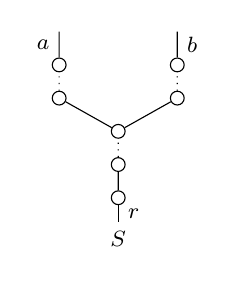
\begin{tikzpicture}
                  [grow=up,auto,
                  level distance=2em,
                  every node/.style = {font=\footnotesize,solid},
                  dummy/.style={circle,draw,inner sep=0pt,minimum size=1.75mm},
                  emph/.style={edge from parent/.style={black,thin,dotted,draw}},
                  norm/.style={edge from parent/.style={black,thin,draw,solid}}
                  ]
                  \node {$S$}
                  child[norm, level distance=1.5em] {node [dummy] {}
                    child[norm, level distance=1.2em] {node [dummy] {}
                      child[emph]{node [dummy] {} % vertex
                        child[norm] {node [dummy] {}
                          child[emph] {node [dummy] {}
                            child[norm] {edge from parent node [swap] {$b$}}
                          }
                        }
                         child[norm] {node [dummy] {}
                          child[emph] {node [dummy] {}
                            child[norm] {edge from parent node {$a$}}
                          }
                        }
                      }
                    }
                    edge from parent node [swap] {$r$}
                  };
            \end{tikzpicture}
      \]
      where there are $n_r$, $n_b$, and $n_a$ edges on the bottom, right, and left paths respectively.
\end{example}
      
Now, $\mathbb F^{\mathbf E(T)}\eta_{\mathbf E(T)}(C) = \varnothing$ unless $C = (e;e)$ for some $e \in \mathbf E(T)$;
in this case, $\mathbb F^{\mathbf E(T)}\eta(e;e) = \mathbb Z_{\geq 0}$, as in \eqref{FET_EE_EQ}.
% 
If we also denote the unit map by $\eta$, we see that the image of the map
\[
      \mathbb F^{\mathbf E(T)}\eta \xrightarrow{\mathbb F^{\mathbf E(T)}\eta} \mathbb F^{\mathbf E(T)} \Omega(T)
\]
corresponds to all factorizations from \eqref{FET_EQ} with $S_1$ a linear tree and $\phi$ (and hence $\psi_1$) a degeneracy.

Thus in the pushout $\mathbb F^{\mathbf E(T)}_+\Omega(T)$, all the non-injective operations are identified, and we have
\begin{align*}
  \mathbb F^{\mathbf E(T)}_+\Omega(T)(C)
  & = \set{\mbox{factorizations $C_n \xrightarrow{\psi_0} S_1 \xrightarrow{\psi_1} T$ of $\phi$ with $\psi_1$ injective, $\psi_0$ tall}} \\
  & = \set{\mbox{inner faces $S$ of $T_{\phi(1 2 \dots n) \leq \phi(0)}$}} \\
  & = \set{\mbox{subsets $S \subseteq \mathbf E^i(T_{\phi(1 2 \dots n) \leq \phi(0)})$ of inner edges}}    
\end{align*}
where $1 2 \dots n \leq 0$ is the vertex of $C_n$ and $T_{\phi(1 2 \dots n) \leq \phi(0)}$ is the associated outer face of $T$.

In a similar fashion,
% ---------------------------------------- OLIVE GREEN ----------------------------------------
{\color{OliveGreen} using concatinations of pushout squares of the form
  \[
        \begin{tikzcd}
              \mathbb F^2 \eta \arrow[r] \arrow[d]
              &
              \mathbb F \eta \arrow[d] \arrow[r]\
              &
              \eta \arrow[d]
              \\
              \mathbb F X \arrow[r]
              &
              \mathbb F( \mathbb F_+ X) \arrow[r]
              &
              \mathbb F_+^2 X,
        \end{tikzcd}
  \]
} % ---------------------------------------- OLIVE GREEN ----------------------------------------
  we see that
\begin{align*}
  \left(\mathbb F^{\mathbf E(T)}\right)^n \Omega(T)(C)
  & = \set{
    \begin{array}{l}
      \mbox{factorizations $C_n \xrightarrow{\psi_0} S_1 \xrightarrow{\psi_1} S_2 \xrightarrow{\psi_2} \dots \xrightarrow{\psi_{n-1}} S_n \xrightarrow{\psi_n} T$}
      \\
      \mbox{of $\phi$ with $\psi_i$ tall for $i < n$}
    \end{array}
  },
  \\
  \left(\mathbb F^{\mathbf E(T)}_+ \right)^2 \Omega(T)(C)
  & = \set{
    \begin{array}{l}
      \mbox{factorizations $C_n \xrightarrow{\psi_0} S_1 \xrightarrow{\psi_1} S_2 \xrightarrow{\psi_2} \dots \xrightarrow{\psi_{n-1}} S_n \xrightarrow{\psi_n} T$}
      \\
      \mbox{of $\phi$ with $\psi_i$ injective for $i > 1$ and $\psi_i$ tall for $i < n$}
    \end{array}
  }
  \\
  &= \set{\mbox{nested subsets $S_1 \subseteq S_2 \subseteq \dots \subseteq S_n \subseteq \mathbf E^i(T_{\phi(1 2 \dots n) \leq \phi(0)})$ of inner edges}}.
\end{align*}

Finally, for any finite set $A$, we recall that the $n$-simplicies of $\Delta[1]^{\times A}$ correspond to $(n+1)$-strings of nested subsets of $A$.
Thus we have the following description of $W(T)$:

\begin{equation}
      \label{WT_EQ}
      W(T)(C) = 
      \begin{cases}
            \Delta[1]^{\times \mathbf E^i(T_{\underline e \leq e})}, \qquad & \mbox{there exist $C_n \xrightarrow{\phi} T$ with $\partial \phi = C$}
            \\
            \varnothing & \text{else,}
      \end{cases}
\end{equation}

It is clear that $W(-)$ is functorial. Thus we have the following definition.

\begin{definition}
      The \textit{homotopy coherent dendroidal nerve} and the \textit{$W_!$-construction}
      are the right- and left-adjoints of the nerve-realization adjunction associated to the functor $W: \Omega \into \Op(\sSet)$.
      \begin{equation}
            \label{SOPDSET_EQ}
            hc N \colon \sOp \leftrightarrows
            \dSet \colon W_!
      \end{equation}
\end{definition}
The culmination of extensive work by Cisinski-Moerdijk-Weiss \cite{CM13a,CM13b,CM11,MW09,MW07} is the following.

\begin{theorem}
      \label{CMW_THM}
      $hcN$ and $W_!$ form a Quillen equivalence with respect to the model structures
      which, in particular, are recovered by the $G = \**$ cases of Theorem \ref{MODEL_THM} and \cite[Thm. 2.1]{Per_eds}.
\end{theorem}

\subsection{The equivariant adjunction}

The main goal of this project \cite{BP_geo,BP_edss,Per_eds} is to understand the correct equivariant lifting of Theorem \ref{CMW_THM}.
On the one hand, the construction of the new adjunction is immediate:

\begin{definition}
      Define
      \[
            W_! \colon \dSet^G \rightleftarrows \sOp^G \colon hcN_d
      \]
      to be the
      extension of the adjunction \eqref{SOPDSET_EQ}
      given by post-composition.
\end{definition}

% Equivalently, given decompositions $T \simeq G \cdot_H U$ and $T \simeq G \cdot U / N$, we have
% $W(T) \simeq G \cdot_H W(U)$ and $W(T) \simeq G \cdot W(U)/N$.


On the other hand, the homotopy theories involved are much more involved to capture the genuine equivariance,
as noted in \cite[\S \ref{GSOP-MSC_SEC}, \S \ref{GSOP-MS_SEC}]{BP_GSOP},
\S \ref{EDS_SEC}, and \cite{Per_eds}.

We have the following generalization of \cite[Prop 4.5]{CM11} (see also \cite[Prop. 6.15]{Per_eds}).

\begin{proposition}
      \label{W!_COF_PROP}
      Suppose $\F = \set{\F_n}$ is a weak indexing system.
      Then $W_!: \dSet^G \to \sOp^G$ sends $\F$-normal monomorphisms to cofibrations and inner $\F$-anodyne extensions to trivial $\F$-cofibrations.
\end{proposition}
\begin{proof}
      It suffices to check this on the generating maps.
      To that end, let $T \in \Omega_F$, choose a decomposition $T \simeq G \cdot_H T_e$ and consider the map
      \begin{equation}
            G \cdot_H \left( W_! \partial \Omega[T_e] \xrightarrow{\ i \ } W(T_e) \right)      
      \end{equation}
      in $\sOp^G$.
      If $T_e = \eta$, then $i$ is the canonical map $\varnothing \to \eta$,
      % W_! \partial \Omega[\eta] = \varnothing \to W(\eta) = \eta$,
      and so $G \cdot_H i$ is a generating cofibration from \eqref{IFJF_EQ} in $\sOp^G$.

      Thus we may assume that $|V(T)| \geq 1$.
      In this case, $i$ is an isomorphism on object $H$-sets $\mathbf E(T_e)$,
      and for any $\mathbf E(T_e)$-signature $C$,
      $i(C)$ is the identity unless $C = h \cdot \mathsf{lr}(T_e)$ for some $h \in H$,
      where $\mathsf{lr}(T_e)$ is the signature $(e_1, \dots, e_n; e)$ 
      with $\set{e_1,\dots, e_n}$ the set of leaves of $T_e$ and $e$ the root.
      When $C = \mathsf{lr}(T_e)$, $i(C)$ is the iterated pushout product
      \[
            i(C) = (\partial \Delta[1] \to \Delta[1])^{\square \mathbf E^i(T_e)}.
      \]
      We need that $i(C)$ is a genuine cofibration in $\sSet^{\Aut(C)}_\F$.
      However, $\Aut(C) = \Gamma \leq H \times \Sigma_n$ for $\Gamma \leq H \times \Sigma_n$ the graph subgroup encoding the $H$-action on the set of leaves $\set{e_1, \dots, e_n}$,
      and since $\F$ is a weak indexing system, $\Aut(C) \in \F_n$,
      and thus, as $\F$ is closed under subgroups, $\sSet^{\Aut(C)}_\F = \sSet^{\Aut(C)}_{gen}$.
      Then the claim follows from the fact that monomorphisms are genuine cofibrations,
      {\color{OliveGreen} % ---------- OLIVE GREEN ----------------------------------------
        or using the fact that $\sSet$ has cofibrant symmetric pushout powers,
        so $(\partial \Delta[1] \to \Delta[1])^{\square m}$ is a genuine $\Sigma_m$-cofibration where $m = |\mathbf E^i(T_e)|$,
        and then as restriction is left Quillen on genuine model structures,
        \[
              \mathrm{Res}^{\Sigma_m}_{\Aut(C)}(\partial \Delta[1] \to \Delta[1])^{\square m} = i(C),
              \qquad
              \Aut(C) = \Gamma \xrightarrow{pr} H \xrightarrow{\mathbf E^i(T_e)} \Sigma_m,
        \]
        is a genuine $\Aut(C)$-cofibration.
      } % ---------------------------------------- OLIVE GREEN --------------------
      %
      It is then straightforward to check that $G \cdot_H i$ has the left lifting property against all local trivial $\F$-fibrations in $\sOp^G$.
      {\color{OliveGreen} % ----------------------------------------
        Indeed, we clearly have a lifts on the level of sequences.
        To check that the resulting map is operadic, it suffices to check on composites of the form
        $C_0 \circ (C_1, \dots, C_n) = \mathsf{lr}(T_e)$.
        If $C_j = \mathsf{lr}(T_e)$ for some $j$, then the composite map is just the identity, and there is no content to check.
        If $C_j \neq \mathsf{lr}(T_e)$ for all $j$,
        then this follows by a simple diagram chase on the cube relating the compositions in $W(T)$ and $W_! \partial \Omega(T)$ with those in the source and target of the testing trivial fibration.
      } % COLOR OLIVEGREEN
      Hence $G \cdot_H i$ is an $\F$-cofibration in $\sOp^G$ by Lemma \ref{CAV_4.8}.
      
     
      Similarly, consider a generating $\F$-inner horn inclusion
      \[
            G \cdot_H \left(W_! \Lambda^{H e}[T_e] \xrightarrow{\ j \ } W(T_e) \right).
      \]
      with $T \simeq G \cdot_H T_e \in \Omega_\F$ and $e \in \mathbf E(T_e)$ some inner edge.
      Again, $j$ is bijective on objects and $j(C)$ is the identity unless $C = h \cdot \mathsf{lr}(T_e)$.
      When $C = \mathsf{lr}(T_e)$, $j(C)$ is the iterated pushout product
      \begin{equation}
            j(C) =
            \left(
                  \begin{tikzcd}
                        \partial \left(
                              \Delta[1]^{\times \mathbf E^i(T_e) \setminus H e}
                        \right) \arrow[d]
                        \\
                        \Delta[1]^{\times \mathbf E^i(T_e) \setminus H e}
                  \end{tikzcd}
            \right) \square
            \left(
                  \begin{tikzcd}
                        \set{1} \arrow[d]
                        \\
                        \Delta[1]
                  \end{tikzcd}
            \right)^{\square H e}
            =
            \left(
                  \begin{tikzcd}
                        \partial \Delta[1] \arrow[d]
                        \\
                        \Delta[1]
                  \end{tikzcd}
            \right)^{\square \mathbf E^i(T_e) \setminus H e}
            \square
            \left(
                  \begin{tikzcd}
                        \set{1} \arrow[d]
                        \\
                        \Delta[1]
                  \end{tikzcd}
            \right)^{\square H e}.                              
      \end{equation}
      A similar argument shows that $G \cdot_H j$ has the left lifting property against all local $\F$-fibrations,
      hence is a trivial $\F$-cofibration in $\sOp^G$ by Lemma \ref{CAV_4.3}, as desired. 
\end{proof}

We have the following immediate corollary.
\begin{corollary}
      [{cf. \cite[Prop. 6.15]{Per_eds}, \cite[Cor. 4.6]{CM11}}]
      For any $\F$-fibrant $\O \in \sOp^G$, $h c N \O$ is an $\F$-$\infty$-operad.
\end{corollary}

Another corollary is the following key step.

\begin{proposition}[{cf. \cite[Prop/ 4.9]{CM11}}]
      $W_!: \dSet^G \to \sOp^G$ is left Quillen.
\end{proposition}
\begin{proof}
      As we already know by Proposition \ref{W!_COF_PROP} that $W_!$ preserves cofibrations,
      it suffices by Corollary \ref{SIMPLQUILL COR} to show that $h c N$ preserves fibrations between fibrant objects.
      Suppose $f: \O \to \P$ is an $\F$-fibration between $\F$-fibrant operads in $\sOp^G$.
      Then Proposition \ref{W!_COF_PROP} also implies that $h c N (f)$ is an $\F$-inner-fibration between $\F$-$\infty$-operads.
      By \cite[Thm. 8.22]{Per_eds}, this is an $\F$-fibration in $\dSet^G_\F$ iff $\tau (h c N_d(f)^H) = \tau (h c N_d(f^H))$ is a categorical fibration for all $H \leq G$.
      But by Remark \ref{FIB_ISOFIB_REM}, being a fibration in $\sOp^G_\F$ implies that $\pi_0(f^H)$ is a categorical fibration for all $H \leq G$, 
      and since $\pi_0 = \tau \circ h c N$ by \cite[Prop. 4.8]{CM11}, the result follows.
\end{proof}

\begin{remark}
      One can also show a more powerful equivariant version of \cite[Prop. 4.8]{CM11},
      namely that the following diagram commutes.
      \begin{equation}
            \begin{tikzcd}
                  \sOp^G \arrow[r, "i_{\**}"] \arrow[d, "h c N"']
                  &
                  \sOp_G \arrow[d, "h c N"] \arrow[r, "\pi_0"]
                  &
                  \Op_G \arrow[d, equal]
                  \\
                  \dSet^G \arrow[r, "i_{\**}"]
                  &
                  \dSet_G \arrow[r, "\tau_G"]
                  &
                  \Op_G
            \end{tikzcd}
      \end{equation}
      In particular, this recovers that $\pi_0 \circ (-)^H = \tau \circ h c N \circ (-)^H$ for all $H$,
      but also more subtle information about the interaction of $\pi_0$ and $h c N$ with the graph subgroup fixed points.
      This story, along with colored genuine equivariant operads as well as cofibrancy considerations of the above narrative,
      will be further explored in a sequel. 
\end{remark}


\todo[inline]{include Proposition \ref{COMUOTOHOM PROP}!}

here!

Finally, the following is a reformalized proof of \cite[Thm. 8.14]{CM13b}, extended to the equivariant setting;
the main result is an immediate corollary.

\begin{proposition}\label{COMUOTOHOM PROP}
      For all weak indexing systems $\F$,
      the (right) derived composite functors in the following diagram commute up to a zigzag of weak equivalences. 
      \[
            \begin{tikzcd}
                  \mathsf{PreOp} \ar{d}[swap]{\gamma^{\**}}&
                  \mathsf{sOp} \ar{l}[swap]{N} \ar{d}{hcN}
                  \\
                  \mathsf{sdSet} &
                  \mathsf{dSet} \ar{l}{c_{!}}
            \end{tikzcd}
      \]
\end{proposition}

Note that though $\gamma^{\**}$ and $c_{!}$ are left Quillen, they both preserve all equivalences, 
so that one needs only perform fibrant replacements in 
$\mathsf{sOp}$.

\begin{proof}
	Recall that, given an object $X$ in a model category $\mathcal{M}$, a simplicial frame of $X$ is a fibrant replacement
	$c_!(X) \to \widetilde{X}(\bullet)$ of the constant 
	simplcial object $c_!(X)$ in the Reedy model structure on $\mathcal{M}^{\Delta^{op}}$.
	Moreover, if $X$ was already fibrant one is free to assume that $\widetilde{X}(0) = X$.
	
	Let $\mathcal{O} \in \mathsf{sOp}$ be fibrant, 
	choose a (functorial) fibrant simplicial frame
	$\widetilde{\mathcal{O}}(\bullet) \in \mathsf{sOp}^{\Delta^{op}}$, where we assume $\widetilde{\mathcal{O}} (0) = \mathcal{O}$.
	Next, let 
	$\gamma^{\**} N \widetilde{\mathcal{O}}(\bullet) 
	\to \widetilde{Q}(\bullet)$
	be a Reedy fibrant replacement in  
	$\mathsf{sdSet}^{\Delta^{op}}$.
	
	We claim that the following is a zigzag of weak equivalences in $\mathsf{sdSet}$.
\begin{equation}\label{BIGZIG EQ}
	\gamma^{\**} N \mathcal{O} \xrightarrow{\sim}
	\widetilde{Q}(0) \xrightarrow{\sim}
	\delta^{\**} \widetilde{Q} \xleftarrow{\sim}
	\widetilde{Q}_0 \xleftarrow{\sim}
	\left(\gamma^{\**} N \widetilde{\mathcal{O}}\right)_0
	\xrightarrow{\sim}
	hcN \widetilde{\mathcal{O}} \xleftarrow{\sim}
	c_{!} hcN \mathcal{O}
\end{equation}
That the first map is an equivalence is obvious from definition of $\widetilde{Q}$ and the assumption $\widetilde{\mathcal{O}}(0) = \mathcal{O}$.

For the second and third maps, note first that $\widetilde{Q}$ is homotopically constant, in the sense that all structure maps $\widetilde{Q}(m) \to \widetilde{Q}(m')$
are equivalences.
Moreover, since the levels $\widetilde{Q}$ are fibrant in 
$\mathsf{sdSet}$, this implies that these are simplicial equivalences, i.e. that for each tree $T \in \Omega$
the evaluations 
$\widetilde{Q}(T)(m) \to \widetilde{Q}(T)(m')$
are Kan equivalences in $\mathsf{sSet}$.
But since $\widetilde{Q}(T) \in \mathsf{sSet}^{\Delta^{op}}$ is itself Reedy fibrant, this shows that it is in fact joint Reedy fibrant, so that one has Kan equivalences 
$\widetilde{Q}(T)(0) \xrightarrow{\sim}
\delta^{\**} \widetilde{Q}(T) \xleftarrow{\sim}
\widetilde{Q}_0(T)$, showing that the second and third maps in \eqref{BIGZIG EQ} are indeed weak equivalences.

For the fourth equivalence, note that one can write
\[\widetilde{Q}_0(T) = 
\mathsf{Hom}_{\mathsf{sdSet}}(\Omega[T],\widetilde{Q})=
\mathsf{Hom}_{\mathsf{PreOp}}(\Omega[T],\gamma_{\**}\widetilde{Q})\]
\[
\left(\gamma^{\**} N \widetilde{\mathcal{O}}\right)_0(T) = 
\mathsf{Hom}_{\mathsf{sdSet}}(\Omega[T],\gamma^{\**} N \widetilde{\mathcal{O}})=
\mathsf{Hom}_{\mathsf{PreOp}}(\Omega[T], N \widetilde{\mathcal{O}})
\]
The claim now follows by noting that
$N \widetilde{\mathcal{O}} \to \gamma_{\**} \widetilde{Q}$
is an equivalence of Reedy fibrant objects on 
$\mathsf{PreOp}^{\Delta^{op}}$ (over the tame model structure) and that $\Omega(T)$ is tame cofibrant. 

For the fifth equivalence, note that
\[
\left(\gamma^{\**} N \widetilde{\mathcal{O}}\right)_0(T) = 
\mathsf{Hom}_{\mathsf{PreOp}}(\Omega[T], N \widetilde{\mathcal{O}}) =
\mathsf{Hom}_{\mathsf{sOp}}(\Omega(T),  \widetilde{\mathcal{O}})
\]
\[
\left(hcN \widetilde{\mathcal{O}} \right)(T) = 
\mathsf{Hom}_{\mathsf{sOp}}(W_!(T),  \widetilde{\mathcal{O}})
\]
so that the required claim follows since 
$\widetilde{\mathcal{O}}$ is Reedy fibrant and
$W_!(T) \to \Omega(T)$ is a weak equivalence of cofibrant operads.

Lastly, for the last map, one needs simply note that
$c_! hcN \mathcal{O} = hcN c_! \mathcal{O}$, so that the required claim follows since 
$c_! \mathcal{O} \to \widetilde{O}$
is a levelwise equivalence of levelwise fibrant operads
and $hcN$ is right Quillen.
\end{proof}

\begin{proof}
      [Proof of Theorem \ref{QE_THM}]
      Proposition \ref{COMUOTOHOM PROP} implies that $W_!$ is an equivalence of homotopy theories.
      Since by Proposition \ref{W!_COF_PROP} it is left Quillen,
      the result follows.
\end{proof}


\section{Indexing system analogue results}

As in \cite[\S 6]{BP_edss} and \cite[\S 9]{Per_eds}, we dedicate our final section to 
outlining the variations of the main results from Sections \ref{TAME_SEC} to
the \textit{indexing systems} of Blumberg-Hill \cite{BH15}, or more accurately
the mild generalization of \textit{weak indexing systems} of the authors \cite[\S 9]{Per_eds}, \cite[\S4.4]{BP_geo} (and independently identified by Gutierrez-White \cite{GW}).

here!




%%%%%%%%%%%%%%%%%%%%%%%%%%%%%%%%%%%%%%%%%%%%%%%%%%%%%%%%%%%%%%%%%%%%%%%
% -------------------- UP: PETER, DOWN: LUIS  --------------------
%%%%%%%%%%%%%%%%%%%%%%%%%%%%%%%%%%%%%%%%%%%%%%%%%%%%%%%%%%%%%%%%%%%%%%%

\newpage

\section{In $\mathsf{dSet}_G$}

\begin{definition}
      Define the \textit{genuine operadic nerve} $N: \Op_G \to \dSet_G$ by
      \begin{equation}
            N\P(T) = \Hom_{\Op_G}(T, \P)
      \end{equation}
      where we think of $T$ as the operad $T \in \Op^G \into \Op_G$. 
\end{definition}

\begin{remark}
      We note that $N\P \in (SCI)^{\boxslash !}$,
      as $T \in \Op_G$ is a free $\mathbb F_G$-algebra on its vertices.
\end{remark}

\begin{remark}
      We can rephrase the definition of being an $\mathbb F_G$-algebra in terms of $N\P$.
      For $\P \in \Sym_G$ a $G$-symmetric sequence,
      a genuine $G$-operad structure on $\P$ is given by:
      \begin{itemize}
      \item Composition Maps: $ $\\
            maps 
            $N\P(T) \to \P(\mathsf{lr}(T))$
            for all $T \in \Omega_G$.
      \item Naturality under restriction and conjugation: $ $\\
            maps $N\P(T_1) \to N\P(T_0)$
            for all quotient maps $T_0 \to T_1$ in $\Omega_{G,0}$,
            such that the following commutes:
            \begin{equation}
                  \begin{tikzcd}
                        N\P(T_1) \arrow[r] \arrow[d]
                        &
                        \P(\mathsf{lr}(T_1)) \arrow[d]
                        \\
                        N\P(T_0) \arrow[r]
                        &
                        \P(\mathsf{lr}(T_0)).
                  \end{tikzcd}
            \end{equation}
      \item Associativity under $\mathbb F_G$: $ $\\
            maps $N\P(T_1) \to N\P(T_0)$
            for all planar tall maps $T_0 \to T_1$ in $\Omega_G^t$,
            such that the analogus diagram (with the right vertical map the identity) commutes.\footnote{
              As in \cite{BP_geo}, we note that ``associativity'' under $\mathbb F_G$ includes both
              the usual notion of associativity of our composition maps,
              but also unitality;
              this is recorded here by the fact that degeneracies are always planar tall.}
      \end{itemize}
\end{remark}

The above reflects the following result.

\begin{proposition}
      $\Op_G$ is equivalent to the subcategory of $\mathsf{dSet_G}$ spanned by those $X$ such that
      \begin{enumerate}
      \item $X(H/H) = \set{\**}$ for all $H \leq G$.
      \item $X(T) \cong \otimes_{T_v \in V(T)}X(T_v)$. 
      \end{enumerate}
\end{proposition}
\begin{proof}
      The fact that $N\P \in (SCI_{\F})^{\boxslash !}$ is immediate, as remarked above.

      For the reverse direction, we will follow the construction of the homotopy operad as in \cite[\S 6]{MW09},
      replacing their use of inner horn inclusions with \textit{orbital} inner $G$-horn inclusions,
      to show that any $X \in (OHI)^{\boxslash !}$ is in the image of $N$; 
      the result will then follow from \cite[HYPER PROP]{BP_edss}.

      In fact, interpreting all of their pictures are as \textit{orbital} representations of $G$-trees yields that,
      for all $C \in \Sigma_G$
      \begin{itemize}
      \item $\sim_{G e}$ is an equivalence relation on $X(C)$ for all $Ge \in E_G(C)$.
      \item The relations $\sim_{G e}$ and $\sim_{G e'}$ are equal for all $e,e'\in E(C)$.
      \item $[h] \circ [f] = [h \circ f]$ yields a well-defined composition map.
      \end{itemize}
      \todo[inline]{naturality, associativity of composition}
\end{proof}



\newpage




\section{Scratchwork}

\subsection{Colored simplicial tensors and cotensors}



\[
\begin{tikzcd}
	K \otimes f^{\**} P \ar{r} \ar{ddd}&
	K \otimes f^{\**} \left( (K \otimes P)^K \right) \ar{r}{\simeq} \ar{d}&
	K \otimes \left( f^{\**} (K \otimes P) \right)^K \ar{r} \ar{d} &
	f^{\**} (K \otimes P) \ar{ddd}
\\
	&
	K \otimes f^{\**} \left( (L \otimes P)^K \right) \ar{d}
	\ar{r}{\simeq} &
	K \otimes \left( f^{\**} (L \otimes P) \right)^K
	\ar{d}
\\
	&
	L \otimes f^{\**} \left( (L \otimes P)^K \right)
	\ar{r}{\simeq} &
	L \otimes \left( f^{\**} (L \otimes P) \right)^K
\\
	L \otimes f^{\**} P \ar{r} &
	L \otimes f^{\**} \left( (L \otimes P)^L \right) \ar{r}{\simeq} \ar{u} &
	L \otimes \left( f^{\**} (L \otimes P) \right)^L \ar{r}&
	f^{\**} (L \otimes P)
\end{tikzcd}
\]



\[
\begin{tikzcd}
	K \otimes f^{\**} P \ar{r} \ar{d}&
	K \otimes f^{\**} \left( (K \otimes P)^K \right) \ar{r}{\simeq} &
	K \otimes \left( f^{\**} (K \otimes P) \right)^K \ar{r}  &
	f^{\**} (K \otimes P) \ar{ddd}
\\
	K \otimes \left( (L \otimes f^{\**} P) \right)^L \ar{d} &
	K \otimes \left( (L \otimes f^{\**} \left( (K \otimes P)^K \right)) \right)^L &
\\
	K \otimes \left( (L \otimes f^{\**} P) \right)^K \ar{d} &
	K \otimes \left( (L \otimes f^{\**} \left( (K \otimes P)^K \right)) \right)^K
\\
	L \otimes f^{\**} P \ar{r} &
	L \otimes f^{\**} \left( (L \otimes P)^L \right) \ar{r}{\simeq} &
	L \otimes \left( f^{\**} (L \otimes P) \right)^L \ar{r}&
	f^{\**} (L \otimes P)
\end{tikzcd}
\]




\[
\begin{tikzcd}
	f^{\**} P \ar{rr} \ar{rd} \ar{dd} & &
	f^{\**} \left( (K \otimes P)^K \right) \ar{d} &
	\left( f^{\**} (K \otimes P) \right)^K \ar{l}[swap]{\simeq} \ar{ddd}
\\
	&
	f^{\**} \left( (L \otimes P)^L \right) \ar{r} &
	f^{\**} \left( (L \otimes P)^K \right) 
\\
	\left( L \otimes f^{\**} P \right)^L \ar{r} \ar{d} &
	\left( f^{\**}( L \otimes P ) \right)^L \ar{u}{\simeq} \ar{rrd} 
\\
	\left( L \otimes f^{\**} P \right)^K \ar{rrr} &&&
	\left( f^{\**}( L \otimes P ) \right)^K \ar{uul}[swap]{\simeq}
\end{tikzcd}
\]


\newpage


\subsection{Semi-cofibrantly generated}


The following codifies a formal argument implicit in the proof of \cite[Thm. 7.19]{CM13b}.

\begin{definition}
Given a set $J$ of maps that admit the small object argument, we say that $X \in \mathcal{M}$ is \textit{$J$-fibrant} if $X \to \**$ has the right lifting property against maps in $J$.

Further, given $D$ a class of maps in $\mathcal{M}$,
we write $D_{J\text{-fib}} \subseteq D$ to denote 
the subclass of maps whose target is $J$-fibrant.
\end{definition}

\begin{lemma}\label{SEMICOF LEM}
	Let $\mathcal{M}$ be a model category with $(C,W,F)$
	the corresponding classes of cofibrations, weak equivalences and fibrations. 
	Further, $J$ be a set of maps admitting the small object argument and such that:
\begin{itemize}
	\item[(i)] $J \subseteq C \cap W$;
	\item[(ii)] 
	$\left(J^{\boxslash} \cap W \right)_{J\text{-fib}}
	\subseteq \left( F \cap W \right)_{J\text{-fib}}$.
\end{itemize}
Then one further has that:
\begin{itemize}
	\item[(a)]
	$\left(\prescript{\boxslash}{}{\left(J^{\boxslash}\right)}\right)_{J\text{-fib}}
	= 
	\left( C \cap W \right)_{J\text{-fib}}$;
	\item[(b)]
	$\left(J^{\boxslash} \right)_{J\text{-fib}}
	= F_{J\text{-fib}}$.
\end{itemize}
\end{lemma}

\begin{remark}
Rephrasing (b), one has that the fibrant objects of $\mathcal{M}$ are precisely the $J$-fibrant objects
and thus that the fibrations between fibrant objects are precisely the $J$-fibrations.
\end{remark}

\begin{proof}
	To check (a), recalling first that 
	$\prescript{\boxslash}{}{\left(J^{\boxslash}\right)}$
	is the saturation of $J$, one has that (i) in fact implies 
	$\prescript{\boxslash}{}{\left(J^{\boxslash}\right)}
		\subseteq C \cap W $.
	For the converse direction, given a trivial cofibration
	$A \to Y$ with $J$-fibrant target,
	form the factorization 
	$A \to X \to Y$ as a 
	$J$-cofibration followed by a $J$-fibration. 
	By the first direction the map $A\to X$ is a weak equivalence, and thus by 2-out-of-3 so is $X \to Y$.
	But then by (ii) the map $X \to Y$ is a trivial fibration, so that the lifting below exists,
	showing that $A \to Y$ is a retract of $A \to X$, and thus also in the saturation $\prescript{\boxslash}{}{\left(J^{\boxslash}\right)}$, 
	as desired.
\[
\begin{tikzcd}
	A \ar[>->]{r}{J} \ar[>->]{d}[swap]{\sim}&
	X \ar[->>]{d}{J}
%& &
%	A \ar[>->]{r}{\sim} \ar[>->]{d}[swap]{\sim}&
%	Y \ar[->>]{d}{\sim}
\\
	Y \ar[equal]{r} \ar[dashed]{ru} & Y
%& &
%	X \ar[equal]{r} \ar[dashed]{ru} & X
\end{tikzcd}
\]

To check (b), one direction is again immediate from (i),
since $J^{\boxslash} \supseteq (C \cap W)^{\boxslash} = F$.
For the converse direction, it suffices to show that 
a $J$-fibration $X\to Y$ with $J$-fibrant target has the right lifting property against trivial cofibrations, as on the left diagram below.
After factoring the bottom horizontal map as a $J$-cofibration followed by a $J$-fibration as on the right diagram, it suffices to shows that a lift $B' \to X$ exists.
But since $B'$ is $J$-fibrant, this follows from (a), which shows that the composite $A \to B \to B'$ is a $J$-cofibration.
\[
\begin{tikzcd}
	A \ar{r} \ar[>->]{d}[swap]{\sim}&
	X \ar[->>]{d}{J}
&&
	A \ar{rr} \ar[>->]{d}[swap]{\sim}&&
	X \ar[->>]{d}{J}
\\
	B \ar{r} \ar[dashed]{ru} & Y
&&
	B \ar[>->]{r}[swap]{J} &
	B' \ar[->>]{r}[swap]{J} \ar[dashed]{ru}
	& Y
\end{tikzcd}
\]
\end{proof}

\begin{remark}
	Analyzing the proof above, one is free to replace the class of fibrant objects with any other class that is compatible with $J$-fibrations, in the sense that if 
	$X \to Y$ is a $J$-fibration and $Y$ is in the class, then so is $X$.
\end{remark}





\subsection{Formalizing some stuff}

The following is a reformalized proof of \cite[Thm. 8.14]{CM13b}.


\begin{proposition}\label{COMUOTOHOM2 PROP}
The (right) derived composite functors in the following diagram commute up to a zigzag of weak equivalences. 
\[
\begin{tikzcd}
	\mathsf{PreOp} \ar{d}[swap]{\gamma^{\**}}&
	\mathsf{sOp} \ar{l}[swap]{N} \ar{d}{hcN}
\\
	\mathsf{sdSet} &
	\mathsf{dSet} \ar{l}{c_{!}}
\end{tikzcd}
\]
\end{proposition}

Note that though $\gamma^{\**}$ and $c_{!}$ are left Quillen, they both preserve all equivalences, 
so that one needs only perform fibrant replacements in 
$\mathsf{sOp}$.

\begin{proof}
	Recall that, given an object $X$ in a model category $\mathcal{M}$, a simplicial frame of $X$ is a fibrant replacement
	$c_!(X) \to \widetilde{X}(\bullet)$ of the constant 
	simplcial object $c_!(X)$ in the Reedy model structure on $\mathcal{M}^{\Delta^{op}}$.
	Moreover, if $X$ was already fibrant one is free to assume that $\widetilde{X}(0) = X$.
	
	Let $\mathcal{O} \in \mathsf{sOp}$ be fibrant, 
	choose a (functorial) fibrant simplicial frame
	$\widetilde{\mathcal{O}}(\bullet) \in \mathsf{sOp}^{\Delta^{op}}$, where we assume $\widetilde{\mathcal{O}} (0) = \mathcal{O}$.
	Next, let 
	$\gamma^{\**} N \widetilde{\mathcal{O}}(\bullet) 
	\to \widetilde{Q}(\bullet)$
	be a Reedy fibrant replacement in  
	$\mathsf{sdSet}^{\Delta^{op}}$.
	
	We claim that the following is a zigzag of weak equivalences in $\mathsf{sdSet}$.
\begin{equation}\label{BIGZIG2 EQ}
	\gamma^{\**} N \mathcal{O} \xrightarrow{\sim}
	\widetilde{Q}(0) \xrightarrow{\sim}
	\delta^{\**} \widetilde{Q} \xleftarrow{\sim}
	\widetilde{Q}_0 \xleftarrow{\sim}
	\left(\gamma^{\**} N \widetilde{\mathcal{O}}\right)_0
	\xrightarrow{\sim}
	hcN \widetilde{\mathcal{O}} \xleftarrow{\sim}
	c_{!} hcN \mathcal{O}
\end{equation}
That the first map is an equivalence is obvious from definition of $\widetilde{Q}$ and the assumption $\widetilde{\mathcal{O}}(0) = \mathcal{O}$.

For the second and third maps, note first that $\widetilde{Q}$ is homotopically constant, in the sense that all structure maps $\widetilde{Q}(m) \to \widetilde{Q}(m')$
are equivalences.
Moreover, since the levels $\widetilde{Q}$ are fibrant in 
$\mathsf{sdSet}$, this implies that these are simplicial equivalences, i.e. that for each tree $T \in \Omega$
the evaluations 
$\widetilde{Q}(T)(m) \to \widetilde{Q}(T)(m')$
are Kan equivalences in $\mathsf{sSet}$.
But since $\widetilde{Q}(T) \in \mathsf{sSet}^{\Delta^{op}}$ is itself Reedy fibrant, this shows that it is in fact joint Reedy fibrant, so that one has Kan equivalences 
$\widetilde{Q}(T)(0) \xrightarrow{\sim}
\delta^{\**} \widetilde{Q}(T) \xleftarrow{\sim}
\widetilde{Q}_0(T)$, showing that the second and third maps in \eqref{BIGZIG2 EQ} are indeed weak equivalences.

For the fourth equivalence, note that one can write
\[\widetilde{Q}_0(T) = 
\mathsf{Hom}_{\mathsf{sdSet}}(\Omega[T],\widetilde{Q})=
\mathsf{Hom}_{\mathsf{PreOp}}(\Omega[T],\gamma_{\**}\widetilde{Q})\]
\[
\left(\gamma^{\**} N \widetilde{\mathcal{O}}\right)_0(T) = 
\mathsf{Hom}_{\mathsf{sdSet}}(\Omega[T],\gamma^{\**} N \widetilde{\mathcal{O}})=
\mathsf{Hom}_{\mathsf{PreOp}}(\Omega[T], N \widetilde{\mathcal{O}})
\]
The claim now follows by noting that
$N \mathcal{O} \to \gamma_{\**} \widetilde{Q}$
is an equivalence of Reedy fibrant objects on 
$\mathsf{PreOp}^{\Delta^{op}}$ (over the tame model structure) and that $\Omega(T)$ is tame cofibrant. 

For the fifth equivalence, note that
\[
\left(\gamma^{\**} N \widetilde{\mathcal{O}}\right)_0(T) = 
\mathsf{Hom}_{\mathsf{PreOp}}(\Omega[T], N \widetilde{\mathcal{O}}) =
\mathsf{Hom}_{\mathsf{sOp}}(\Omega(T),  \widetilde{\mathcal{O}})
\]
\[
\left(hcN \widetilde{\mathcal{O}} \right)(T) = 
\mathsf{Hom}_{\mathsf{sOp}}(W_!(T),  \widetilde{\mathcal{O}})
\]
so that the required claim follows since 
$\widetilde{\mathcal{O}}$ is Reedy fibrant and
$W_!(T) \to \Omega(T)$ is a weak equivalence of cofibrant operads.

Lastly, for the last map, one needs simply note that
$c_! hcN \mathcal{O} = hcN c_! \mathcal{O}$, so that the required claim follows since 
$c_! \mathcal{O} \to \widetilde{O}$
is a levelwise equivalence of levelwise fibrant operads
and $hcN$ is right Quillen.
\end{proof}




\begin{lemma} \label{INTER_LEM}
Let $\mathcal{O} \in \mathsf{sOp}$ and let
$g \colon x \to y$ be an equivalence in $\mathcal{O}$.

Then there exists a countable, cofibrant and contractile $H \in \mathsf{sOp}_{\{0,1\}}$ 
and a map 
$\varphi \colon H \to \mathcal{O}$
such that 
$g$ is in the image of $\varphi$. 
\end{lemma}


\begin{proof}
	We start by considering the case where $\mathcal{O}$ is locally fibrant.
	
	$g$ can be regarded as a map
	$[1] \xrightarrow{g} \mathcal{O}$,
	and one thus likewise gets a map
	$\Delta[1] \xrightarrow{g}  hcN \mathcal{O}$
	which is an equivalence in the 
	$\infty$-category $hcN \mathcal{O}$,
	so that one can find a (non-unique) factorization
	$\Delta[1] \to J \to hcN \mathcal{O}$
	which by adjunction yields a factorization
	$[1]=W_!\Delta[1] \to W_! J \to \mathcal{O}$,
	which establishes the desired claim 
	since $W_! J$ is contractible due to 
	Example \ref{WJ EX}.
	
	For a general $\mathcal{O}$, 
	consider first a local fibrant replacement
	$F \colon \mathcal{O} \to \mathcal{O}'$.
	One can hence find a map 
	$W_! J \to \mathcal{O}'$ such that
	$F(g)$ is in its image. 
	We now factor this map as
	$W_! J \xrightarrow{\sim} H \to \mathcal{O}'$
	where the second map is a local fibration.
	
	One can now form a pullback
\[
\begin{tikzcd}
	\tilde{H} \ar{r} \ar{d} & H' \ar{d}
\\
	\mathcal{O} \ar{r} & \mathcal{O}'
\end{tikzcd}
\]
where $\tilde{H}$ is seen to be contractible since
$\mathsf{sSet}$ is right proper.
	A priori, $\tilde{H}$ will need not be countable nor cofibrant, but this is easily rectified:
	indeed one can show that any countable subcomplex of $\tilde{H}$ is contained in a contractible countable subomplex, 
	yielding a countable contractible subcomplex whose image in $\mathcal{O}$ contains $g$. Lastly, performing a cofibrant replacement of that complex finishes the proof.
\end{proof}



\begin{example}\label{WJ EX}
	Let $J = N \widetilde{[1]}$ be the nerve of the contractible groupoid on two objects.
	
	Then there is an identification
\[
	W_{!} J \simeq \mathbb{F}^{\bullet} \widetilde{[1]}
\]
	where $\mathbb{F}$ denotes the (unital) free operad monad.

	To see this, we start by describing
	$\mathbb{F}^{\bullet} \widetilde{[1]}$.
	Writing $f \colon 0 \to 1$ and 
	$g \colon  1\to 0$ for the non-identity arrows in 
	$\widetilde{[1]}$ (so that $g=f^{-1}$), the $0$-simplices of $\mathbb{F}^{\bullet} \widetilde{[1]}$
	are the alternating words
	$f,g,fg,gf,fgf,gfg,fgfg,gfgf,\cdots$
	in the letters $f$, $g$.
	More generally
	$n$-simplices are given by equipping such alternating words with ``$n$ nested layers of brackets''
	(so that, for example, 
	$\left((f)(gf)\right) 
	\left( (gf) \right)$
	encodes a $2$-simplex).
	Alternatively, given an alternating word of length $l$, such bracketings are encoded by a flag of subsets
	$F_1 \subseteq F_2 \subseteq \cdots 
	\subseteq F_n \subseteq \{1,\cdots,l-1\}$.
	
	To describe $W_{!} J$, we apply the explicit description of the $W_{!} (-)$ construction given in 
	\cite{DS11}.
	Following \cite[Cor. 4.8]{DS11}, the $n$-simplices of $W_{!} J$ are uniquely encoded by a map
\begin{equation}\label{NECMAP EQ}
	N = \Delta^{k_1} \vee \Delta^{k_2} 
	\vee \cdots \vee \Delta^{k_r} 
	\to J 
\end{equation}
which is totally nondegenerate (this means that all simplices $\Delta^{k_i} \to J$ are nondegenerate)
together with a flag of subsets
	$\boldsymbol{J}(N) = 
	G_0 \subseteq 
	G_1 \subseteq \cdots \subseteq
	G_{n-1} \subseteq \boldsymbol{E}^{\mathsf{i}}(N)$.
	Noting that the nondegenerate simplices of $J$ (other than the points $0,1$)
	are themselves identified with alternating words
	$f,g,fg,gf,fgf,gfg,fgfg,gfgf,\cdots$,
	one sees that so is the map \eqref{NECMAP EQ}.
	Therefore, we see that a $n$-simplex of 
	$W_{!} J$ is uniquely, determined by some alternating word of some size $l$ together with a flag  
	$G_0 \subseteq 
	G_1 \subseteq \cdots \subseteq
	G_{n-1} \subseteq \boldsymbol{E}^{\mathsf{i}}(N)
	=\{1,\cdots,l-1\}$, since 
	$G_0$ suffices to recover the domain of 
	\eqref{NECMAP EQ}.
	
	This shows that $W_{!} J$ $\mathbb{F}^{\bullet} \widetilde{[1]}$ indeed have the same simplices.
	The fact that the simplicial operators coincide can be readily checked explicitly with the most interesting case is that of the top differential $d_n$, which in either case is induced by multiplication in 
	$\widetilde{[1]}$ 
	(that this is the case for $W_{!} J$ follows from the description of the simplicial operators in 
	\cite[Cor. 4.4]{DS11} together with the description of the ``flanking'' procedure in \cite[Lemma 4.5]{DS11}).
\end{example}




\subsection{Extra lifts for $\infty$-categories}


\begin{lemma}
The inclusion 
\[[0,1,2] \cup [0,2,3,\cdots,n] \cup 
\Lambda^0[0,1,3,\cdots,n]
 \to \Lambda^{0,2}[n]\]
is built cellularly from inclusions
$\Lambda^0[k] \to \Delta[k]$ with $k<n$.
Moreover, all such cells send $[0,1]$ to $[0,1]$.
\end{lemma}

\begin{proof}
Since $[0,2,3,\cdots,n]$ is in the domain, all missing faces must contain $1$.
Moreover, since the smallest face not containing $2$
that is not in $\Lambda^0[0,1,3,\cdots,n]$ is $[1,3,\cdots,n]$,
which is also the smallest face not in $\Lambda^{0,2}[n]$,
we see that all missing faces must contain $2$ as well.

It now suffices to check that $0$ is characteristic with respect to the missing faces, i.e.
that $12\underline{a}$ is missing iff $012\underline{a}$ is missing, and this is now obvious. 
\end{proof}

\begin{remark}
	The map $\Lambda^{0,2}[n] \to \Delta[n]$ is inner anodyne ($2$ is characteristic).
	
	This observation, together with the precious lemma, are the technical core of the observation that lifts
\[
	\begin{tikzcd}
	\Lambda^{0}[n] \ar{d}  \ar{r} & X
\\
	\Delta[n] \ar[dashed]{ru}
	\end{tikzcd}
\]
exist when $X$ is an $\infty$-category and $[0,1]$ is mapped to an equivalence in $X$.
\end{remark}




\subsection{TBD}


\begin{lemma}
Suppose that a subcategory $\Xi$ has subcategories 
$\Xi^-,\Xi^+$ which contain the isomorphisms and satisfy the unique factorization up to unique isomorphism axiom.

Write $\mathsf{Arr}(\Xi)$ for the arrow category of $\Xi$ and 
$\mathsf{Arr}^{-}(\Xi), \mathsf{Arr}^{+}(\Xi)$
for the full subcategories whose objects are arrows in $\Xi^-,\Xi^+$. 
Then $\mathsf{Arr}^{-}(\Xi)$ (resp. $\mathsf{Arr}^{+}(\Xi)$)
is initial (resp. terminal) in $\mathsf{Arr}(\Xi)$.
\end{lemma}



\begin{proof}
Given $f \in \mathsf{Arr}(\Xi)$, we need to show that there exist diagrams as on the left, and moreover that all such diagrams are connected. 
Existence is immediate from the factorization assumption . Moreover, its is straightforward from the ``uniqueness up to isomorphism'' that all connections are connected.
But by factoring the left vertical map in the diagram below, we now see that all such diagrams are connected to a factorization.
\[
\begin{tikzcd}
	\bullet \ar{r}{f} \ar{d}& 
	\bullet \ar{d}
\\
	\bullet \ar{r}[swap]{+} &
	\bullet
\end{tikzcd}
\]
%
%\[
%\begin{tikzcd}
%	\bullet \ar{r}{-} \ar{dd} \ar{rd}[swap]{-} &
%	\bullet \ar{rrr}{+} \ar{rrd}{-} &&&
%	\bullet \ar{dd}
%\\
%	&
%	\bullet \ar{rrd}[swap]{+}  && 
%	\bullet \ar{rd}{+} \ar[dashed]{ll}[swap]{\simeq}
%\\
%	\bullet 	\ar{rrr}[swap]{-} &&&
%	\bullet \ar{r}[swap]{+} & 
%	\bullet
%\end{tikzcd}
%\]
\end{proof}



\begin{lemma}\label{REDUCELAN LEM}
	Suppose that $F \colon \mathcal{C} \to \mathcal{D}$ is a functor in 
	$\mathsf{Cat}^G$.
Then the following square commutes up to natural isomorphism
\[
\begin{tikzcd}[column sep=50pt]
	\mathcal{V}^{G \ltimes \mathcal{C}} 
	\ar{r}{\mathsf{Lan}_{G \ltimes \mathcal{C} \to G \ltimes \mathcal{D}}} \ar{d}[swap]{\mathsf{fgt}}&
	\mathcal{V}^{G \ltimes \mathcal{D}} \ar{d}{\mathsf{fgt}}
\\
	\mathcal{V}^{\mathcal{C}} 
	\ar{r}[swap]{\mathsf{Lan}_{\mathcal{C} \to\mathcal{D}}} &
	\mathcal{V}^{\mathcal{D}}
\end{tikzcd}
\]
\end{lemma}


\begin{proof}
For each $d \in \mathcal{D}$ (recall that $\mathcal{D}$ and $G \ltimes \mathcal{D}$ have the same objects) one has an obvious inclusion 
$\mathcal{C} \downarrow d \to G\ltimes \mathcal{C} \downarrow d$.
Moreover, for each object of $G\ltimes \mathcal{C} \downarrow d$
there is a unique $g \in G$ such that the object is described as a composite
$F(c) \xrightarrow{g} g F(c) \to d$,
were $g F(c) \to d$ can be regarded as an object of $\mathcal{C} \downarrow d$.
One thus has a retraction 
$G \ltimes \mathcal{C} \downarrow d \to \mathcal{C} \downarrow d$
showing that $\mathcal{C} \downarrow d$ is terminal in
$G \ltimes \mathcal{C} \downarrow d$
and finishing the proof. 
\end{proof}



\subsection{Fixed color lemmas}

Given a set $\mathfrak{C}$ of colors,
write $\Sigma_{\mathfrak{C}}$ for the groupoid of corollas with edges labeled by colors in $\mathfrak{C}$.

If, in addition, $\mathfrak{C}$ is a $G$-set, 
we write $G \ltimes \Sigma_{\mathfrak{C}}^{op}$ for the larger groupoid obtained via the associated Grothendieck construction.


Writing
$\mathsf{Sym}^{G,\mathfrak{C}} = 
\mathsf{Set}^{G \ltimes \Sigma_{\mathfrak{C}}^{op}}$,
we have a natural monad $\mathbb{F}$ on
$\mathsf{Sym}^{G,\mathfrak{C}}$
whose algebra category we denote by 
$\mathsf{Op}^{G,\mathfrak{C}}$.


\begin{notation}
	Given a $G$-equivariant function 
	$f \colon \mathfrak{C} \to \mathfrak{D}$
	we write
\[
	f_{\**} \colon 
	\mathsf{Sym}^{G,\mathfrak{C}}
	\rightleftarrows
	\mathsf{Sym}^{G,\mathfrak{D}}
	\colon f^{\**}
\qquad
	\check{f}_{\**} \colon 
	\mathsf{Op}^{G,\mathfrak{C}}
	\rightleftarrows
	\mathsf{Op}^{G,\mathfrak{D}}
	\colon f^{\**}
\]
for the standard adjunctions (note the need to distinguish notations for the left adjoints).
\end{notation}


\begin{example}\label{GCORMPA EX}
Given a $G$-corolla $C \in \Sigma_G$, we write $\partial C$ for the set of edges of $C$, which is naturally identified with the set of objects of the associated $G$-operad
$\Omega(C) \in \mathsf{Op}^G$.

One can then regard $\Omega(C) \in \mathsf{Op}^{G,\partial C}$ and, moreover, $\Omega(C)$ is in fact the free operad over the symmetric sequence obtained by removing the units of $\Omega(C)$,
which we denote by
$\Omega'(C) \in \mathsf{Sym}^{G,\partial C}$.

Given the non-equivariant decomposition
$C = C_1 \amalg \cdots \amalg C_k$
with $C_i \in \Sigma$, 
one can naturally regard the $C_i$ as objects of $\Sigma_{\partial C}$.
In fact, one then has an identification
\begin{equation}\label{SOMEIDEN EQ}
	\Omega'(C) \simeq 
	\Sigma_{\partial C}[C_1] \amalg \cdots \amalg \Sigma_{\partial C}[C_k]
\end{equation}
where $\Sigma_{\partial C}[-]$ denotes the representable presheaf in 
$\mathsf{Set}^{\Sigma_{\partial C}^{op}}$.
This claim requires some justification, since a priori the right hand side of \eqref{SOMEIDEN EQ} is an object in $\mathsf{Set}^{\Sigma_{\partial C}^{op}}$,
rather than in $\mathsf{Set}^{G \ltimes \Sigma_{\partial C}^{op}}$,
i.e. we need to describe the action of the additional action arrows
$D \xrightarrow{g} gD$ on this presheaf.
This action is given by the following diagram, where the vertical $g$ arrows simply act on labels, and all horizontal arrows are shuffle arrows (i.e. arrows in $\Sigma_{\partial C}$).
The diagonal $C_g$ arrow corresponds to the structural $G$-action on $C$. It is then straightforward to check that there is a unique dashed shuffle $\tau_g$ as indicated
\[
\begin{tikzcd}
	D \ar{d}[swap]{g} \ar{r}{\sigma} & C_i \ar{rd}{C_g} \ar{d}[swap]{g}
\\
	g D \ar{r}[swap]{g \sigma} & g C_i \ar[dashed]{r}{\simeq}[swap]{\tau_g} & C_{g i}
\end{tikzcd}
\]
and one defines $g_{\**}\colon \Sigma_{\partial C}[C_i] \to \Sigma_{\partial C}[C_{gi}]$
via $\sigma \mapsto \tau_g \circ (g \sigma)$.

Moreover, letting $f \colon \partial C \to \mathfrak{C}$
be a map of colors, 
one obtains $\mathfrak{C}$-corollas $C_i^{f} \in \Sigma_{\mathfrak{C}}$
by coloring each edge $e\in \partial C$ by $f(e) \in \mathfrak{C}$, resulting in a generalized identification 
\begin{equation}\label{SOMEIDENGEN EQ}
	f_{\**} \Omega'(C) \simeq 
	\Sigma_{\mathfrak{C}}[C_1^f] \amalg \cdots \amalg \Sigma_{\mathfrak{C}}[C^f_k]
\end{equation}
Indeed, \eqref{SOMEIDENGEN EQ} follows from the observation
that the Kan extension 
$\mathsf{Lan}_{G \ltimes \Sigma_{\partial C} \to G \ltimes \Sigma_{\mathfrak{C}}}$ 
coincides, after forgetting with the $G$-action arrows,
with the Kan extension
$\mathsf{Lan}_{\Sigma_{\partial C} \to \Sigma_{\mathfrak{C}}}$
(cf. Lemma \ref{REDUCELAN LEM}).
\end{example}


\begin{definition}
      \label{COR_GGRAPH_DEF}
	Given a $\mathfrak{C}$-corolla $C$, 
	a subgroup 
	$\Gamma \leq \mathsf{Aut}_{G \ltimes \Sigma_{\mathfrak{C}}^{op}}(C)$
	is called a \textit{$G$-graph subgroup} if
	$\Gamma \cap \mathsf{Aut}_{\Sigma_{\mathfrak{C}}^{op}}(C) = \**$.
	
	We write $\mathcal{F}^{\Gamma} = \{\mathcal{F}^{\Gamma}_C\}$
	for the collection of families of $G$-graph subgroups.
	
	A $G$-$\mathfrak{C}$-symmetric sequence
	$X \in \mathsf{Sym}^{G,\mathfrak{C}}$
	is called $\Sigma$-cofibrant if each level
	$X(C)$ is $\mathcal{F}^{\Gamma}_C$-cofibrant.
\end{definition}


\begin{remark}
	Write a $\mathfrak{C}$-corolla as $C^f \in \Sigma_{\mathfrak{C}}$,
	where $C \in \Sigma$ is the underlying corolla and
	$f\colon \partial C \to \mathfrak{C}$
	is the coloring.
	A $G$-graph subgroup 
	$\Gamma \leq \mathsf{Aut}_{G \ltimes \Sigma_{\mathfrak{C}}^{op}}(C^f)$ is, under the map 
	$G \ltimes \Sigma_{\mathfrak{C}}^{op} \to
	G \times \Sigma^{op}$,
	identified with a 
	$G$-graph subgroup of 
	$G \times \mathsf{Aut}_{\Sigma^{op}}(C)$,
	i.e., with the graph of a partial antihomomorphism
\[
	G^{op} \geq H^{op} \xrightarrow{(-)^{-1}} H 
	\xrightarrow{\tau_{(-)}} \mathsf{Aut}_{\Sigma^{op}}(C)
\]
	which is subject to the requirement
\[
	f(\tau_h(e)) = h f(e).
\]
Using the $\tau$ automorphisms one can then
\begin{inparaenum}
\item[(i)] equip $C$ with a $H$-action,
so that one can regard $C \in \Sigma^H \subseteq \Sigma_H$;
\item[(ii)] extend $\Sigma_{\mathfrak{C}}[C^f]$ to 
an object in $\mathsf{Set}^{H \ltimes \Sigma_{\mathfrak{C}}}$
by defining the action of the $H$-action arrows $h$ via 
$\sigma \mapsto \tau_{h} \circ (h \sigma)$;
\item[(iii)]
following Example \ref{GCORMPA EX}, one thus has an identification
\[
	f_{\**} \Omega'(C) \simeq \Sigma_{\mathfrak{C}}[C^f]
\]
of objects in $\mathsf{Set}^{H \ltimes \Sigma_{\mathfrak{C}}}$ and therefore an identification 
\[
	f_{\**} \left( G \cdot_H \Omega'(C) \right) \simeq 
	G\cdot_H \Sigma_{\mathfrak{C}}[C^f]
\]
of objects in $\mathsf{Set}^{G \ltimes \Sigma_{\mathfrak{C}}}$.
\end{inparaenum}
\end{remark}


\begin{example}
Let $G = \mathbb{Z}_{/2} = \{\pm 1\}$ and 
$\mathfrak{C} = \{\mathfrak{a}, -\mathfrak{a}, \mathfrak{b}\}$ where we implicitly have
$-\mathfrak{b} = \mathfrak{b}$.
Consider the two $\mathfrak{C}$-corollas 
$C,D \in \Sigma_{\mathfrak{C}}$ below.
\begin{equation}
	\begin{tikzpicture}[auto,grow=up, level distance = 2.2em,
	every node/.style={font=\scriptsize,inner sep = 2pt}]%
		\tikzstyle{level 2}=[sibling distance=3em]%
			\node at (0,0) [font = \normalsize] {$C$}%	
				child{node [dummy] {}%
					child{node {}%
					edge from parent node [swap] {$-\mathfrak{a}$}}%
					child[level distance = 2.9em]{node {}%
					edge from parent node [swap,	near end] {$\mathfrak{b}$}}%
					child[level distance = 2.9em]{node {}%
					edge from parent node [near end] {$\mathfrak{b}$}}%
					child{node {}%
					edge from parent node  {$\mathfrak{a}$}}%
				edge from parent node [swap] {$\mathfrak{b}$}};%
			\node at (7,0) [font = \normalsize] {$D$}%	
				child{node [dummy] {}%
					child{node {}%
					edge from parent node [swap] {$-\mathfrak{a}$}}%
					child[level distance = 2.9em]{node {}%
					edge from parent node [swap,	near end] {$-\mathfrak{a}$}}%
					child[level distance = 2.9em]{node {}%
					edge from parent node [near end] {$\mathfrak{a}$}}%
					child{node {}%
					edge from parent node  {$\mathfrak{a}$}}%
				edge from parent node [swap] {$\mathfrak{b}$}};%
	\end{tikzpicture}%
\end{equation}%
Each of $C,D$ admit exactly two non-trivial $G$-graph subgroups,
which are encoded by the $\mathbb{Z}_{/2}$-actions on the underlying corollas depicted below.
\begin{equation}
	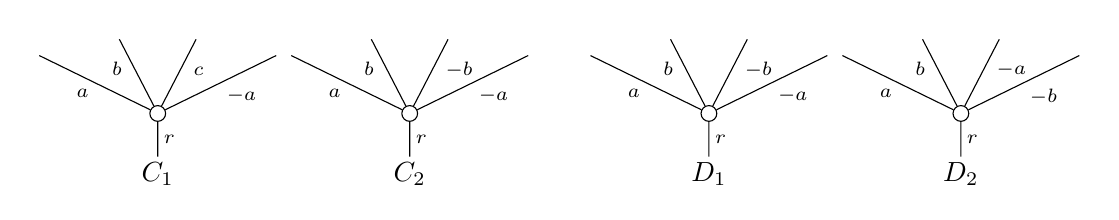
\begin{tikzpicture}[auto,grow=up, level distance = 2.2em,
	every node/.style={font=\scriptsize,inner sep = 2pt}]%
		\tikzstyle{level 2}=[sibling distance=3em]%
			\node at (-1.6,0) [font = \normalsize] {$C_1$}%	
				child{node [dummy] {}%
					child{node {}%
					edge from parent node [swap] {$-a$}}%
					child[level distance = 2.9em]{node {}%
					edge from parent node [swap,	near end] {$c\phantom{b}$}}%
					child[level distance = 2.9em]{node {}%
					edge from parent node [near end] {$b$}}%
					child{node {}%
					edge from parent node  {$a$}}%
				edge from parent node [swap] {$r$}};%
			\node at (1.6,0) [font = \normalsize] {$C_2$}%	
				child{node [dummy] {}%
					child{node {}%
					edge from parent node [swap] {$-a$}}%
					child[level distance = 2.9em]{node {}%
					edge from parent node [swap,	near end] {$-b$}}%
					child[level distance = 2.9em]{node {}%
					edge from parent node [near end] {$b$}}%
					child{node {}%
					edge from parent node  {$a$}}%
				edge from parent node [swap] {$r$}};%
			\node at (5.4,0) [font = \normalsize] {$D_1$}%	
				child{node [dummy] {}%
					child{node {}%
					edge from parent node [swap] {$-a$}}%
					child[level distance = 2.9em]{node {}%
					edge from parent node [swap,	near end] {$-b$}}%
					child[level distance = 2.9em]{node {}%
					edge from parent node [near end] {$b$}}%
					child{node {}%
					edge from parent node  {$a$}}%
				edge from parent node [swap] {$r$}};%
			\node at (8.6,0) [font = \normalsize] {$D_2$}%	
				child{node [dummy] {}%
					child{node {}%
					edge from parent node [swap] {$-b$}}%
					child[level distance = 2.9em]{node {}%
					edge from parent node [swap,	near end] {$-a$}}%
					child[level distance = 2.9em]{node {}%
					edge from parent node [near end] {$b$}}%
					child{node {}%
					edge from parent node  {$a$}}%
				edge from parent node [swap] {$r$}};%
	\end{tikzpicture}%
\end{equation}%

\end{example}


The following is the analogue of \cite[Prop. 3.2]{CM13b}

\begin{proposition}\label{KEYPR PROP}
Suppose that $\mathcal{O} \in \mathsf{Op}^{G,\mathfrak{C}}$
is $\Sigma$-cofibrant.
Further, let $C \in \Sigma_G$ be any $G$-corolla and consider 
a pushout in $\mathsf{Op}^{G}$ of the form
\begin{equation}\label{PUSHOUTPROP EQ}
\begin{tikzcd}
	\partial \Omega(C) \ar{r} \ar{d} & \mathcal{O} \ar{d}
\\
	\Omega(C) \ar{r} & \mathcal{P}.
\end{tikzcd}
\end{equation}
Then the induced map
\begin{equation}\label{ANODYNE MAP}
	\Omega[C] \amalg_{\partial \Omega[C]} N\mathcal{O} \to N\mathcal{P}
\end{equation}
is $G$-inner anodyne.
\end{proposition}

\begin{proof}
The desired claim that \eqref{ANODYNE MAP}
is $G$-inner anodyne will follow by applying the  
\textit{characteristic edge lemma} \cite[Lemma 3.4]{BP_edss},
but we first need some preliminary discussion. 

Let us write $f \colon \partial C \to \mathfrak{C}$
for the induced map of colors.
The first step is to rewrite \eqref{PUSHOUTPROP EQ} as a pushout diagram in $\mathsf{Op}^{G,\mathfrak{C}}$, which can be done by applying $\check{f}_{\**}$
to the leftmost objects in \eqref{PUSHOUTPROP EQ}.
Since
\[
	\check{f}_{\**} \Omega(C) \simeq 
	\check{f}_{\**} \left( \mathbb{F} \Omega'(C) \right) \simeq 
	\mathbb{F} \left(f_{\**}  \Omega'(C) \right)
\]
one has that, writing $C \simeq G \cdot_H C_{\star}$ one has the alternative pushout in $\mathsf{Op}^{G,\mathfrak{C}}$
\begin{equation}
\begin{tikzcd}
	\mathbb{F} ( \emptyset ) \ar{r} \ar{d} & \mathcal{O} \ar{d}
\\
	\mathbb{F} \left( 
	G \cdot_H \Sigma_{\mathfrak{C}}[C^f_{\star}] \right) \ar{r} & \mathcal{P}.
\end{tikzcd}
\end{equation}
Writing $B = G \cdot_H \Sigma_{\mathfrak{C}}[C^f_{\star}]$, one then has
\begin{equation}\label{PUSHOPPR EQ}
	\mathcal{P}(C) = 
	\coprod_{
	[T] \in \mathsf{Iso}
	\left( \Omega_{\mathfrak{C}}^a \downarrow_{\mathsf{r}} C \right)
	}
	\left(
		\prod_{v \in V^{ac}(T)} \mathcal{O}(T_v)
	\times
		\prod_{v \in V^{in}(T)} B(T_v)
	\right)
	\cdot_{\mathsf{Aut}_{\Omega^a_{\mathfrak{C}}}(T)} \mathsf{Aut}_{\Sigma_{\mathfrak{C}}}(C)
\end{equation}

We now discuss the dendrices of $N \mathcal{P}$. Firstly, recall that, by the strict Segal condition characterization of nerves \cite[Cor. 2.7]{CM13a},
a dendrex $\Omega[T] \to N \mathcal{P}$
is uniquely specified by the tree $T \in \Omega$ together with a choice of operations
$\{p_v \in \mathcal{P}(T_v)\}_{v \in \boldsymbol{V}(T)}$.
Noting that \eqref{PUSHOPPR EQ} implies that the canonical map (of sequences) 
$\mathcal{O} \amalg B \to \mathcal{P}$
is a monomorphism, 
we will say a dendrex $(T,\{p_v\})$ is \textit{elementary}
if all operations $p_v$ are in $\mathcal{O} \amalg B$.
Additionally, an elementary dendrex $(T,\{p_v\})$ is called \textit{alternating} if $T$ is an alternating tree and 
$p_v$ is in $\mathcal{O}$ (resp. $B$) if
$v \in \boldsymbol{V}(T)$ is active (resp. inert).

Given an elementary dendrex $(T,\{p_v\})$ and a map of trees 
$\varphi \colon S \to T$
we will need to know when 
$\varphi^{\**}(T,\{p_v\})$
is again elementary.
Since all maps in $\Omega$ are, uniquely up to isomorphism,
factored as a degeneracy followed by an inner face followed by an outer face, it suffices to discuss each of those cases.
It is straightforward to check that 
$\varphi^{\**}(T,\{p_v\})$ 
is elementary whenever $\varphi$ is a degeneracy or an outer face.
For an inner face
$\varphi \colon T-D \to T$,
noting that a partial composite $p \circ_i q$ of non-unit operations is in $\mathcal{O} \amalg B$ iff both operations are in $\mathcal{O}$,
one sees that $\varphi^{\**}(T,\{p_v\})$ is elementary iff
for each $d \in D$ the adjacent vertices of $T$ are either both labeled by operations of $\mathcal{P}$ or one of them is labeled by an identity.
An elementary dendrex is called \textit{reduced} if it has no such edges. 
In other words, an elementary dendrex is reduced iff none of its inner faces are reduced, so that, in particular, all elementary dendrices admit at least one reduced inner face (note that specifying such a face is somewhat subtle: even when a dendrex is non-degenerate, it may not be enough to collapse edges connecting $\mathcal{O}$ vertices, since this may possibly introduce new identity vertices, resulting in a degenerate vertex).
Note that reduced dendrices are necessarily non-degenerate, but not vice versa.
In fact, a non-degenerate dendrex is reduced iff it has a degeneracy which is an alternating dendrex. 


In what follows, we will find it convenient to work with elementary dendrices that have been suitably ``planarized''.
To do so, fix a subset
$\mathcal{O}^{\mathsf{st}} \amalg B^{\mathsf{st}} 
\subset
\coprod_{C \in \Sigma_{\mathfrak{C}}}
\mathcal{O}(C) \amalg B(C)$
of coset representatives for the $\Sigma$-action,
which we call \textit{standard} representatives.
An elementary dendrex $(T,\{p_v\})$ is then called \textit{standard}
if all $p_v$ are standard (i.e. in 
$\mathcal{O}^{\mathsf{st}} \amalg B^{\mathsf{st}}$).
Moreover, since both $\mathcal{O}$ and $B$ are $\Sigma$-cofibrant/$\Sigma$-free sequences (the former by assumption),
for each elementary simplex $(T,\{p_v\})$,
there is a unique (replanarization) isomorphism
$\varphi \colon T' \to T$ such that
$(T',\{\varphi^{\**}p_v\})$ is standard,
and we write 
$\mathsf{st}(T,\{p_v\}) = \varphi^{\**} (T,\{p_v\}) = (T',\{\varphi^{\**}_v p_v\})$
to denote this.


Note that it now follows from \eqref{PUSHOPPR EQ} that,
for each operation $p \in \mathcal{P}(C)$,
there exists a unique standard alternating dendrex
$b'_p \colon \Omega[T'_p] \to N \mathcal{P}$ and isomorphism 
$C \simeq T'_p - \boldsymbol{E}^{\mathsf{i}}(T'_p)$
such that the composite
\begin{equation}\label{STANDELDE EQ}
	\Omega[C] \simeq
	\Omega[T'_p - \boldsymbol{E}^{\mathsf{i}}(T'_p)] \to 
	\Omega[T'_p] \xrightarrow{b'_p}
	N \mathcal{P}
\qquad
	\Omega[C] \simeq
	\Omega[T_p - \boldsymbol{E}^{\mathsf{i}}(T_p)] \to 
	\Omega[T_p] \xrightarrow{b_p}
	N \mathcal{P}
\end{equation}
is $p$. In fact, due to the correspondence between alternating elementary dendrices and reduced elementary dendrices, 
the analogous claim  also holds 
for the corresponding non-degenerate dendrex 
$b_p \colon \Omega[T_p] \to N \mathcal{P}$.


We can now finally discuss how to apply \cite[Lemma 3.4]{BP_edss}.

Firstly, we need to identify a $G$-poset $I$ and dendrices 
$b_i \colon \Omega[U_i] \to N \mathcal{P}$ for $i \in I$.
Firstly, the underlying set of $I$ is the set of 
non-degenerate standard dendrices of $\mathcal{P}$,
which we abbreviate as
$i = (U_i,\{p_v^i\})$.
The dendrex $b_i \colon \Omega[U_i] \to N \mathcal{P}$ is then tautological, being $i$ itself, but it will preferable to use distinct notations for $i \in I$ and
$b_i \in N \mathcal{P} (U_i)$.
Given $i,j \in I$, we write $i \leq j$ if exists a (in general not  planar) face map
$\varphi \colon U_i \to U_j$
such that $b_i = \varphi^{\**}(b_j)$.
Note that by the uniqueness of standardizations $\varphi$ can only be an isomorphism if $i=j$, showing that $\leq$ indeed satisfies anti-symmetry.
Lastly, we define the $G$-action on $I$ via
\[b_{g i} = \mathsf{st} (g b_i).\]
When reading this formula, note that
$g b_i \in \mathcal{P}(U_i)$
(since this uses the $G$-action
on $\mathcal{P}$),
while $b_{g i} \in \mathcal{P}(U_{g i})$,
where $U_{g i}$ comes with the unique isomorphism
$U_{g i} \xrightarrow{g^{-1}} U_i$ which standardizes $b g_i$.

Lastly, the characteristic edge sets 
$\Xi^i \subseteq \boldsymbol{E}^{\mathsf{i}}(U_i)$ consist of those inner edges such that at least one of the adjacent vertices is mapped to an operation in $B$. Note that, by the discussion above, for an inner face of $\varphi \colon U_i - D \to U_i$
the dendrex $\varphi^{\**}(b_i)$ is elementary iff
$D \cap \Xi^i = \emptyset$.

We now note that it is in fact 
$N \mathcal{P} = 
A \cup \bigcup_{i \in I} b_i\left(\Omega[U_i]\right)$.
Indeed, given an arbitrary (non-elementary) non-degenerate dendrex
$(S,\{p_v\}_{v \in \boldsymbol{V}(T)})$, 
the trees $T_{p_v}$ from \eqref{STANDELDE EQ}
can be regarded as a $S$-substitution datum, which after assembled
yields a non-degenerate standard dendrex 
$\Omega[T] \xrightarrow{b_{\{p_v\}}} N \mathcal{P}$ 
whose image contains $(S,\{p_v\}_{v})$.

We now check the characteristic conditions in \cite[Lemma 3.4]{BP_edss}.

(Ch0.2) is straightforward.

For (Ch1), since outer faces of standard dendrices are again standard, one needs only consider the case 
$\bar{V}=U_i$, or else $\bar{V}$ would be in some $U_j$ for $j<i$.
But if $\bar{V}=U_i$, the assumption in (Ch1) states that
$\Xi^i = \emptyset$, so that $i$ must either be a dendrex where all vertices map to $\mathcal{O}$, i.e. $b_i \in N \mathcal{O}$,
or $U_i$ is a corolla its vertex maps to $B$, i.e. 
$b_i \in B$.
In either case, one has
$b_i \in A = B \cup N\mathcal{O}$, and (Ch1) follows.

To check both (Ch2) and (Ch3), observe first that
$V \hookrightarrow U_i$ will automatically be in $A_{<i}$ if either 
$\bar{V} \neq U_i$ or $T = U_i - D$ with 
$D \not \subseteq \Xi_i$
(since in either case $U_i$ would be in some $U_j$ with $j<i$),
so that one needs only consider the case 
$V=U_i$.

(Ch2) then follows since, except in the trivial cases where $\Xi^i = \emptyset$, the dendrex $b_i(U_i - \Xi^i)$ always contains at least one vertex not in $\mathcal{O} \amalg B$.

For (Ch3), we argue that if 
$b_i(U_i - \Xi^i) \in b_j \left( \Omega[U_j] \right)$
then in fact $i\leq j$.
Writing $\bar{U}_i = U_i - \Xi^i$, the hypothesis is that
\[
\begin{tikzcd}
	\bar{U}_i \ar{d} \ar{r}{\bar{\varphi}} & U_j \ar{r}{b_j} & N \mathcal{P}
\\
	U_i \ar[dashed]{ru}[swap]{\varphi}
\end{tikzcd}
\]
there is a face map $\bar{\varphi}$ as above such that
$b_i(\bar{U}_i) = \bar{\varphi}^{\**}(b_j)$, and the goal is to build $\varphi$ such that $b_i = \varphi^{\**}(b_j)$.
Let $w \in \boldsymbol{V}(\bar{U}_i)$ be a vertex and 
let $p_w$ be the corresponding operation of $\mathcal{P}$.
Then the outer fact $(U_i)_{w}$ is precisely $T_{p_w}$ from
\eqref{STANDELDE EQ}.
On the other hand, letting
$(U_j)_w - D_w \hookrightarrow (U_j)_w$
be any choice of reduced inner face, 
one has that this too is $T_{p_w}$, at least up to a replanarization isomorphism, i.e. one has isomorphims
$(U_i)_{w} \simeq (U_j)_w - D_w$,
compatible with the restrictions of $b_i$, $b_j$.
But then combining these isomorphisms yields the desired $\varphi$,
and (Ch3) follows.

Lastly, we show (Ch0.1).
Given any non-degenerate dendrex
$\Omega[V] \xrightarrow{c} N \mathcal{P}$
by applying \eqref{STANDELDE EQ} to each individual operation
(together with an ``assembly of substitution data'' argument)
one obtains that there exists a unique
non-degenerate standard dendrex 
$b_c \colon \Omega[U_c] \to N \mathcal{P}$,
edge subset $D_c \subseteq \Xi^c$ and isomorphism
$V \simeq U_c - D_c$
such that $b$ equals the composite
\begin{equation}\label{STANDELDEGER EQ}
	V \simeq U_c - D_c
	\hookrightarrow U_c
	\xrightarrow{b_c} N \mathcal{P}
\end{equation}
Recall now that, by the preliminary argument for (Ch2) and (Ch3), 
the non-degenerate dendrices not in 
$b_i^{-1}(A_{< i})$ are precisely the replanarizations of the faces 
$U_i - D$ with $D \subseteq \Xi^i$.
But the uniqueness of the data in \eqref{STANDELDEGER EQ}
implies that all such replanarizations of the $U_i - D$
do indeed have distinct images in $N \mathcal{P}$,
thus establishing (Ch0.1) and finishing the proof.
\end{proof}


\begin{remark}
	In general, injectivity of the map
	$b_i \colon \Omega[U_i] \to N \mathcal{P}$
	will fail in $b_i^{-1}(A_{< i})$.
	Indeed, in general two edges/vertices of $U_i$
	may be assigned the same color/operation of $\mathcal{P}$.
	In fact, injectivity may in general fail even for large outer faces.
\end{remark}


{\color{blue} Bla poset not finite but still projective/injective, which is enough}


\begin{remark}
In addition to \eqref{PUSHOPPR EQ}, 
one also has the alternative formula
\begin{equation}\label{PUSHOPPRG EQ}
	\mathcal{P}(C) = 
	\coprod_{
	[T] \in \mathsf{Iso}
	\left( G \ltimes \Omega_{\mathfrak{C}}^a \downarrow_{\mathsf{r}} C \right)
	}
	\left(
		\prod_{v \in V^{ac}(T)} \mathcal{O}(T_v)
	\times
		\prod_{v \in V^{in}(T)} B(T_v)
	\right)
	\cdot_{\mathsf{Aut}_{G \ltimes \Omega^a_{\mathfrak{C}}}(T)} \mathsf{Aut}_{G \ltimes \Sigma_{\mathfrak{C}}}(C)
\end{equation}
which replaces the roles of 
$\Omega_{\mathfrak{C}}^a$, $\Sigma_{\mathfrak{C}}$
with 
$G \ltimes \Omega_{\mathfrak{C}}^a$,
$G \ltimes \Sigma_{\mathfrak{C}}$.
The connection between the two formulas is given by Lemma \ref{REDUCELAN LEM},
though some care is needed.
Namely, \eqref{PUSHOPPRG EQ} generally features fewer coproduct summands but this is compensated by the inductions
$(-) \cdot_{\mathsf{Aut}_{G \ltimes \Omega^a_{\mathfrak{C}}}(T)} \mathsf{Aut}_{G \ltimes \Sigma_{\mathfrak{C}}}(C)$,
which produce more terms than the 
$(-) \cdot_{\mathsf{Aut}_{\Omega^a_{\mathfrak{C}}}(T)} \mathsf{Aut}_{\Sigma_{\mathfrak{C}}}(C)$
inductions.
\end{remark}



\subsection{Tame time}

\begin{definition}
	The \textit{colored tensor product} 
\[
\begin{tikzcd}[row sep = 0, column sep = 40pt]
	\mathsf{PreOp}^G \times \mathsf{sSet} \ar{r}{(-)\otimes_{\mathfrak{C}}(-)} &
	\mathsf{PreOp}^G
\end{tikzcd}
\]
is defined by $(X \otimes_{\mathfrak{C}} K)(T) = X(T) \times K$
whenever $T$ is a non-linear tree (equivalently, 
$\mathsf{Hom}_{\Omega}(T,\eta)=\emptyset$) and
is defined by the following pushout when $T=[n]$ is linear.
\[
\begin{tikzcd}
	X(\eta) \times K \ar{r} \ar{d} \arrow[dr, phantom, "\ulcorner", very near start]  &
	X(\eta) \ar{d}
\\
	X([n]) \times K \ar{r} & 
	(X \otimes_{\mathfrak{C}} K)([n]) 
\end{tikzcd}
\]
\end{definition}

\begin{remark}
More concisely, $X \otimes_{\mathfrak{C}} K$ is defined by the pushout
\[
\begin{tikzcd}
	\left(\mathsf{sk}_{\eta}X \right) \times K \ar{r} \ar{d} \arrow[dr, phantom, "\ulcorner", very near start]  &
	\mathsf{sk}_{\eta}X \ar{d}
\\
	X \times K \ar{r} & 
	X \otimes_{\mathfrak{C}} K 
\end{tikzcd}
\]
\end{remark}


\begin{remark}
For fixed $K \in \mathsf{sSet}$, the functor
$(-) \otimes_{\mathfrak{C}} K
\colon \mathsf{PreOp}^G \to \mathsf{PreOp}^G$
preserves all colimits (indeed, it is not hard to build the right adjoint explicitly).

However, for a fixed $X \in \mathsf{PreOp}^G$,
the functor 
$X \otimes_{\mathfrak{C}} (-)
\colon \mathsf{sSet} \to \mathsf{PreOp}^G$
does not preserve all colimits.
In particular, this functor can not preserve coproducts since, writing 
$\mathcal{C} = X(\eta)$ for the $G$-set of objects of $X$,
the image of $X \otimes_{\mathfrak{C}} (-)$ is entirely contained in the subcategory
$\mathsf{PreOp}^{G,\mathfrak{C}} \subset
\mathsf{PreOp}^G$
of preoperads with $G$-set of objects $\mathfrak{C}$ and maps which are the identity on objects. 
Instead, one has that the functor 
\[
X \otimes_{\mathfrak{C}} (-) \colon
\mathsf{sSet} \to \mathsf{PreOp}^{G,\mathfrak{C}}
\]
does preserve colimits. 
In practice, this means that some standard arguments concerning tensor products can only be applied after adjusting the objects of the relevant preoperads
({\color{red} see later}).
\end{remark}


\begin{remark}\label{COLORTENSGAM REM}
Let $X \to Y$ be any map in $\mathsf{PreOp}^G$
which is the identity on colors and 
$K \in \mathsf{sSet}$. Then the squares below are pushout squares.
Moreover, whenever $K$ is connected the rightmost horizontal maps are isomorphisms.
\[
\begin{tikzcd}
	X \times K \ar{r} \ar{d} 
	\arrow[dr, phantom, "\ulcorner", very near start] &
	\gamma_! \left( X \times K \right) \ar{r} \ar{d} 
	\arrow[dr, phantom, "\ulcorner", very near start] &
	X \otimes_{\mathfrak{C}} K \ar{d}
\\
	Y \times K \ar{r} &
	\gamma_! \left( Y \times K \right) \ar{r} &
	Y \otimes_{\mathfrak{C}} K
\end{tikzcd}
\]
\end{remark}


\begin{definition}
	Let $f \colon \mathfrak{C} \to \mathfrak{D}$
	be a map of $G$-sets (of colors).
	We define adjoint functors
\[
	f_{!} \colon
	\mathsf{PreOp}^{G,\mathfrak{C}}
\rightleftarrows
	\mathsf{PreOp}^{G,\mathfrak{D}}
	\colon f^{\**}
\]
via the pushout and pullback squares
(note that $\mathsf{sk}_{\eta} f_! A$ depends only on 
$\mathfrak{C}$ while 
$\mathsf{csk}_{\eta} f^{\**} X$ depends only on
$\mathfrak{D}$)
\[
\begin{tikzcd}
	\mathsf{sk}_{\eta} A \ar{r} \ar{d} \arrow[dr, phantom, "\ulcorner", very near start]  &
	\mathsf{sk}_{\eta} f_! A \ar{d}
&&
	f^{\**} X \ar{r} \ar{d} &
	X \ar{d}
\\
	A \ar{r} & 
	f_! A
&&
	\mathsf{csk}_{\eta} f^{\**} X \ar{r} & 
	\mathsf{csk}_{\eta} X
	\arrow[ul, phantom, "\lrcorner", very near start]
\end{tikzcd}
\]
\end{definition}


\begin{definition}
	A $G$-preoperad $X \in \mathsf{PreOp}^G$ is called a \textit{$G$-Segal operad} if, 
	for each $G$-tree $T$,
	the natural map 
	$X\left( \Omega[T] \right) \to 
	X \left( Sc[T] \right)$
	is a Kan equivalence.
\end{definition}

\begin{notation}
Given a $G$-Segal operad $X$ and $G$-corolla $C$, 
$X(\partial \Omega[C])$ is a discrete simplicial set whose elements
are the $C$-signatures $(c_1,\cdots,c_n;c_0)$ of $X$.
The map $X(\Omega[C]) \to X(\partial \Omega[C])$ hence yields
a coproduct decomposition 
\[
X(\Omega[C]) \simeq \coprod_{C\text{-signatures }(c_1,\cdots,c_n;c_0)}
X(c_1,\cdots,c_n;c_0)
\]
\end{notation}


\begin{remark}\label{SEOPDK REM}
Given a $G$-Segal operad $X$, consider a dendroidal Reedy fibrant replacement $X \to \tilde{X}$ such that $X(\eta) \simeq \tilde{X}(\eta)$. 
This means that all maps 
$X(\Omega[T]) \to \tilde{X}(\Omega[T])$ are Kan equivalences,
and moreover, by the following pullback diagram
\[
\begin{tikzcd}
	Z (Sc[T]) \ar{r} \ar{d} &
	\prod_{v \in \boldsymbol{V}_G(T)} Z
	(\Omega[T_v]) \ar{d}
\\
	\prod_{(G/H_i \cdot e_i) \in \boldsymbol{E}_G(T)} 
	\mathfrak{C}^{H_i} \ar{r}  &
	\prod_{v \in \boldsymbol{V}_G(T)}
	\prod_{(G/H_i \cdot e_i) \in \boldsymbol{E}_G(T_v)} 
	\mathfrak{C}^{H_i} 
	\arrow[ul, phantom, "\lrcorner", very near start]
\end{tikzcd}
\]
so are the maps $X(Sc[T]) \to \tilde{X}(Sc[T])$.
This shows that $\tilde{X}$ is also a Segal operad, 
and thus a fibrant object in $\mathsf{PreOp}^G$.

Furthermore, the Kan equivalences 
$X(\Omega[C]) \to \tilde{X}(\Omega[C])$
induce Kan equivalences 
$X(c_1,\cdots,c_n;c_0) \to \tilde{X}(c_1,\cdots,c_n;c_0)$.
It follows that the complete equivalences between Segal operads are precisely the Dwyer-Kan equivalences. 
\end{remark}


\begin{remark}\label{SLIMOD REM}
Noting that for every fibrant 
$\tilde{X} \in \mathsf{PreOp}^G$
any equivalence in $\tilde{X}$ is in the image of a map
$J \to \tilde{X}$, 
a slight modification of the proof of Lemma \ref{INTER_LEM}
shows that for any Segal operad $X$
any equivalence in $X$ is in the image of a countable, contractible
$I \in \mathsf{PreOp}^G$
such that $\eta \amalg \eta \to I$
is a tame cofibration.
\end{remark}




\begin{theorem}
	There is a model structure on 
	$\mathsf{PreOp}^G$,
	called the \textbf{tame model structure},
	such that:
\begin{itemize}
	\item the weak equivalences are the complete equivalences (i.e. detected by inclusion into 
	$\mathsf{sdSet}^G$);
	\item generating cofibrations are given by the maps
	\begin{itemize}
		\item[(TC1)] $G/H \cdot \left(\emptyset \to\Omega[\eta]\right)$ for $H\leq G$;
		\item[(TC2)] $\Omega[C] \otimes_{\mathfrak{C}} \left(\partial \Delta[n] \to \Delta[n]\right)$ for $C \in \Sigma_G$, $n \geq 0$;
		\item[(TC3)] 
$\left( Sc[T] \to \Omega[T] \right) 
\square_{\mathfrak{C}} 
\left(\partial \Delta[n] \to \Delta[n]\right)$ for $T \in \Omega_G$, $n \geq 0$.
	\end{itemize}
\end{itemize}
Furthermore, one has generating anodyne cofibrations the maps
\begin{itemize}
	\item[(TA1)] $G/H \cdot 
	\left(\Omega[\eta] \to I \right)$ for $H \leq G$,
	and $\Omega[\eta] \to I$ a weak equivalence in $\mathsf{PreOp}$ such that $I(\eta) = \{0,1\}$, $\Omega[\eta] \amalg \Omega[\eta] \to I$ is a tame cofibration, and $I$ is countable;
	\item[(TA2)] $\Omega[C] \otimes_{\mathfrak{C}}\left(\Lambda^i[n] \to \Delta[n]\right)$ for $C \in \Sigma_G$, $0 \leq i \leq n$;
	\item[(TA3)] 
$\left( Sc[T] \to \Omega[T] \right) 
\square_{\mathfrak{C}} 
\left(\partial \Delta[n] \to \Delta[n]\right)$ for $T \in \Omega_G$, $n \geq 0$.
	\end{itemize}
\end{theorem}


\begin{proof}
	The existence of the model structure will follow by applying J. Smith's theorem \cite[Thm. 1.7]{Bek00}. Conditions c0 and c2 therein are inherited from $\mathsf{sdSet}^G$
	and the technical ``solution set condition'' c3 follows from
	\cite[Prop. 1.15]{Bek00} since weak equivalences are accessible, being the preimage by $\gamma^{\**}$ if the weak equivalences in 
	$\mathsf{sdSet}^G$ 
	(see \cite[Cor. A.2.6.5]{Lur09} and \cite[Cor. A.2.6.6]{Lur09}).
	
	For c1, we must show that any map $X \to Y$ with the right lifting property against (TC1), (TC2), (TC3) is a weak equivalence.
	Writing $f \colon \mathfrak{C} \to \mathfrak{D}$ for the underlying map of colors,
	consider the factorization $X \to f^{\**}Y \to Y$.
	Note that since maps out of (TC1) depend only on objects and both of (TC2) and (TC3) consist of maps which are identities on objects,
	$X \to Y$ will have the right lifting property against (TC1) iff 
	$f^{\**} X \to Y$ does
	and the right lifting property against 
	(TC2) and (TC3) iff $X \to f^{\**}Y$ does.
	
Note now that $f^{\**} Y \to Y$ has the right lifting proper against all maps 
	$\left(\partial \Omega[T] \to \Omega[T] \right) \times \Delta[n]$.
	Indeed, if $T \simeq G/H \cdot \eta$ is a stick, this is precisely the lifting condition agains (TC1), and otherwise it follows automatically since $\left(\partial \Omega[T] \to \Omega[T] \right) \times \Delta[n]$ is the identity on objects.
	Therefore, the levels 
	$\left(f^{\**} Y \right)_n \to Y_n$ are trivial fibrations in 
	$\mathsf{dSet}^G$, showing that 
	$f^{\**} Y \to Y$ is a dendroidal equivalence, 
	and thus a complete equivalence. 
	
	Since the maps in both of (TC2) and (TC3) are the identify on objects, $X \to Y$ has the right lifting property against these maps iff $X \to f^{\**}Y$ does.
The lifting property against (TC2) then says that the maps
$X(\Omega[C]) \to f^{\**} Y (\Omega[C])$
are trivial Kan fibrations for all $G$-corollas $C \in \Sigma_G$,
and thus so are the maps
$X(Sc[T]) \to f^{\**} Y (Sc[T])$ for all $G$-trees $T \in \Omega_G$.
But it then follows from the lifting property against
(TC3) that the maps 
$X(\Omega[T]) \to f^{\**} Y (\Omega[T])$
are trivial Kan fibrations for all $G$-trees,
showing that $X \to f^{\**} Y$ is a simplicial equivalence, and thus a complete equivalence. 
\[
\begin{tikzcd}
	X(\Omega[T]) \ar{r} \ar[->>]{d}{\sim} &
	X(Sc[T]) \ar{r} \ar[->>]{d}{\sim} &
	\prod_{v \in \boldsymbol{V}_G(T)} X(\Omega[T_v])
	\ar[->>]{d}{\sim}
\\
	f^{\**} Y(\Omega[T]) \ar{r} &
	f^{\**} Y(Sc[T]) \ar{r} \ar{d} &
	\prod_{v \in \boldsymbol{V}_G(T)} f^{\**} Y
	(\Omega[T_v]) \ar{d}
	\arrow[ul, phantom, "\lrcorner", very near start]
\\
	&
	\prod_{(G/H_i \cdot e_i) \in \boldsymbol{E}_G(T)} 
	\mathfrak{C}^{H_i} \ar{r}  &
	\prod_{v \in \boldsymbol{V}_G(T)}
	\prod_{(G/H_i \cdot e_i) \in \boldsymbol{E}_G(T_v)} 
	\mathfrak{C}^{H_i} 
	\arrow[ul, phantom, "\lrcorner", very near start]
\end{tikzcd}
\]
This completes the proof of c1, establishing the existence of the tame model structure.

We now turn to the ``further'' claim considering the claimed generating anodyne cofibrations, i.e., 
we wish to show that the maps in 
(TA1), (TA2), (TA3) satisfy the conditions in
Lemma \ref{SEMICOF LEM}.

We first check condition (i).
The case of maps in (TC1) is tautological.
Since $\Lambda^{i}[n]$ is connected, 
the maps in (TA2) have the form
$\gamma_{!} 
\left( \Omega[C] \times
\left( \Lambda^i[n] \to \Delta[n] \right) \right)$,
and are thus weak equivalences thanks to the pushouts
in Remark \ref{COLORTENSGAM REM}.
As for (TA3), it follows from Remark \ref{COLORTENSGAM REM}
that the maps
$\left( Sc[T] \to \Omega[T] \right) \otimes \partial \Delta[n]$
and 
$\left( Sc[T] \to \Omega[T] \right) \otimes \Delta[n]$
are trivial cofibrations, so that the claim follows from a standard pushout and 2-out-of-3 argument.

We now turn to condition (ii).
The lifting condition against (TA3) says that $J$-fibrant objects are such that the maps $X(\Omega[T]) \to X(Sc[T])$
are trivial fibrations, and thus that such $X$ are Segal operads.
Therefore, by Remark \ref{SEOPDK REM} it suffices to check that $J$-fibrations between Segal operads which are also DK equivalences are in fact trivial fibrations, i.e. that they have the right lifting property against the maps in (TC1),(TC2),(TC3).
Given $X \to Y$ a $J$-fibration with $J$-fibrant $Y$,
the lifting property against (TC3) is tautological since 
(TC3) equals (TA3).
Next, the lifting property against (TA2) says that the maps
$X(\Omega[T]) \to f^{\**} Y(\Omega[T])$
are Kan fibrations, and the DK condition says that these are Kan equivalences,
so that we conclude that such maps have the right lifting property against (TC2).
Lastly, given any lifting problem against a map in (TC1),
essential surjectivity and Remark \ref{SLIMOD REM}
produce a lifting problem against a map in (TA1) which has a solution, providing a solution to the original problem.
\end{proof}


{\color{red} To show that maps in (TA3) are normal cofibrations one can use a pushout of projective cofibrant cubes argument.}


The following results are adapted from \cite{JT07} (see Proposition 7.15 therein). 


\begin{proposition}
	A cofibration $A \to B$ is a weak equivalence iff it has the left lifting property against all fibrations between fibrant objects.
\end{proposition}

\begin{proof}
	Let $B \xrightarrow{\sim} \tilde{B}$ be a fibrant replacement and
	let $A \xrightarrow{\sim} \tilde{A} \twoheadrightarrow \tilde{B}$
	be a factorization of the composite $A \to \tilde{B}$ 
	as a trivial cofibration followed by a fibration.
	One then has a lift in the diagram
\[
\begin{tikzcd}
	A \ar{r}{\sim} \ar[>->]{d} & \tilde{A} \ar[->>]{d}
\\
	B \ar{r}{\sim} \ar[dashed]{ru} & \tilde{B}
\end{tikzcd}
\]
where the top and bottom horizontal maps are weak equivalences. 
But then the 2-out-of-6 property for weak equivalences says that all maps are weak equivalences.
\end{proof}


\begin{corollary}\label{SIMPLQUILL COR}
An adjunction 
\[
F \colon \mathcal{C}
	\rightleftarrows
\mathcal{D} \colon G
\]
between model categories is a Quillen adjunction
provided that $F$ preserves cofibrations
and $G$ preserves fibrations between fibrant objects.
\end{corollary}


\begin{lemma}
	Let $A \to B$ be a tame cofibration in $\mathsf{PreOp}^G$, 
	$\mathcal{O} \in \mathsf{sOp}^G$ a $\Sigma$-cofibrant 
	$G$-operad,
	and consider a pushout diagram in $\mathsf{sOp}^G$ of the form
\[
\begin{tikzcd}
	\tau A \ar{r} \ar{d} & \mathcal{O} \ar{d}
\\
	\tau B \ar{r} & \mathcal{P}
\end{tikzcd}
\]
	Then $\mathcal{O} \to \mathcal{P}$ is a $\Sigma$-cofibration and 
\begin{equation}\label{UNITEQUIV EQ}
B \amalg_{A} N \mathcal{O}
	\to 
N \mathcal{P}
\end{equation}
is a weak equivalence.
\end{lemma}

\begin{proof}
	We first consider the case where $A\to B$ is in one of (TC1),(TC2),(TC3). 
	
	The (TC1) case is immediate, 
	since $\mathcal{O} \to \mathcal{O} \amalg G/H \cdot \Omega(\eta)$ is a $\Sigma$-cofibration and
	\eqref{UNITEQUIV EQ}
	is the isomorphism
	$N\mathcal{O} \amalg G/H\cdot \Omega[\eta] \simeq 
	N\left( \mathcal{O} \amalg G/H \cdot \Omega(\eta) \right)$.

	The (TC3) case is also straightforward:
	since $\tau A \to \tau B$ is an isomorphism, one can take 
	$\mathcal{O}=\mathcal{P}$, so that 
	\eqref{UNITEQUIV EQ} becomes a section of the map
	$N \mathcal{O} \to B \amalg_{A} N \mathcal{O}$, which is a trivial cofibration (it is a pushout of $A \to B$),
	and 2-out-of-3 hence implies that \eqref{UNITEQUIV EQ} is a weak equivalence.

	The most interesting case is then (TC2), 
	in which case it is well known that 
	$\mathcal{O} \to \mathcal{P}$ is a $\Sigma$-cofibration and
	each of the levels
$(B \amalg_{A} N \mathcal{O})_n
	\to 
(N \mathcal{P})_n$
for $n \geq 0$
is an equivalence in $\mathsf{dSet}^G$ by (an iteration of)
Proposition \ref{KEYPR PROP}, 
showing that \eqref{UNITEQUIV EQ} is in fact a dendroidal equivalence, and thus also a complete equivalence.

	We now turn to the case of $A \to B$ a general cofibration between cofibrant objects.
	As usual, $A \to B$ is a retract of a transfinite composition of pushouts of generating cofibrations.
	Since the conclusions of the result are invariant under retracts,
	we are free to assume that $A \to B$ is a transfinite composite
\[
A = A_0 \to A_1 \to A_2 \to \cdots \to A_{\beta} \to 
colim_{\beta < \kappa} A_{\beta} = B.
\]
where each map $A_{\beta} \to A_{\beta +1}$ is a pushout of a map in one of (TC1),(TC2),(TC3).

Defining $\mathcal{O}_{\beta}$ by replacing $A \to B$ with $A \to A_{\beta}$ in the pushout,
$\mathcal{O} \to \mathcal{P}$ becomes the transfinite composite of the maps $\mathcal{O}_{\beta} \to \mathcal{O}_{\beta + 1}$
and \eqref{UNITEQUIV EQ} becomes
$
colim_{\beta < \kappa} \left( 
N \mathcal{O} \amalg_{N \tau A} N \tau A_{\beta}
	\to 
N \mathcal{O}_{\beta}
\right)
$.
It thus suffices to show, by induction on $\beta < \kappa$, 
that the maps $\mathcal{O}_{\beta} \to \mathcal{O}_{\beta + 1}$ are $\Sigma$-cofibrations and that the maps 
$N \mathcal{O} \amalg_{N \tau A} N \tau A_{\beta}
	\to 
N \mathcal{O}_{\beta}$
are weak equivalences
(that this last condition suffices follows since
filtered colimits of weak equivalences in $\mathsf{PreOp}^G$ are weak equivalences ({\color{red} add this})).
Consider now the following diagrams.
\[
\begin{tikzcd}
	\tau A \ar{r} \ar{d} & \mathcal{O} \ar{d}
&&
	A_{\beta} \amalg_{A} N \mathcal{O}
	\ar[>->]{r} \ar{d}[swap]{\sim} &
	A_{\beta+1} \amalg_{A} N \mathcal{O}
	\ar{d}[swap]{\sim}
\\
	\tau A_{\beta} \ar{r} \ar{d} & \mathcal{O}_{\beta} \ar{d}
&&
	N \mathcal{O}_{\beta} \ar[>->]{r} &
	A_{\beta+1} \amalg_{A_{\beta}} N \mathcal{O}_{\beta} \ar{d}
\\
	\tau A_{\beta + 1} \ar{r} & \mathcal{O}_{\beta + 1}
&&
	&
	N \mathcal{O}_{\beta+1}
\end{tikzcd}
\]
The induction hypothesis states that
$\mathcal{O} \to \mathcal{O}_{\beta}$ is a $\Sigma$-cofibration and that the map
$A_{\beta} \amalg_A N \mathcal{O} \to \mathcal{O}_{\beta}$ is a weak equivalence.
Therefore, $\mathcal{O}_{\beta}$ is $\Sigma$-cofibrant 
and the both vertical maps marked $\sim$ in the rightmost diagram above are weak equivalences 
(this uses the fact that $\mathsf{PreOp}^G$ is left proper),
and thus the induction step will follow provided that the result holds for
the map $A_{\beta} \to A_{\beta + 1}$ and $\mathcal{O}_{\beta}$.
But $A_{\beta} \to A_{\beta + 1}$ is assumed to be a pushout of a map in (TC1),(TC2),(TC3), in which case the result is already known, and thus noting that the result is clearly invariant under pushouts finishes the proof.
\end{proof}

Setting $A = \emptyset $, $\mathcal{O}= \emptyset$ in the previous result yields the following.

\begin{corollary}\label{KEYEQUIV COR}
	If $B \in \mathsf{PreOp}^G$ is tame cofibrant, then 
	$B \to N \tau B$ is a weak equivalence.
\end{corollary}

\begin{proposition}\label{PREQUIEQUIV PROP}
The adjunction
\[
	\tau \colon \mathsf{PreOp}^G_{\text{tame}}
		\rightleftarrows 
	\mathsf{sOp}^G \colon N
\]
is a Quillen equivalence.
\end{proposition}


\begin{proof}
Firstly, note that $N$ preserves and detects weak equivalences.
Indeed, this follows since all objects in the image of $N$ are Segal operads, so that by Remark \ref{SEOPDK REM} a map in the image of $N$ is a weak equivalence iff it is a Dwyer-Kan equivalence.

Next, we show that this is a Quillen adjunction using Corollary \ref{SIMPLQUILL COR}.
The claim that $\tau$ preserves cofibrations follows since
$\tau$ sends the maps in (TC1) and (TC2) to generating cofibrations of $\mathsf{sOp}^G$ and the maps in (TC3) to isomorphisms.
For the claim that $N$ preserves fibrations between fibrant,
we use a somewhat indirect argument
(though we note that a direct argument is also possible,
by showing that fibrations between fibrant objects in $\mathsf{PreOp}^G$
also satisfy a ``local fibration plus isofibration'' description).
By Corollary \ref{KEYEQUIV COR} and 2-out-of-3, 
one has that for any trivial cofibration between cofibrant objects
$A \to B$, the map $N \tau A \to N \tau B$ is a weak equivalence, and thus so is $\tau A \to \tau B$.
This shows that $\tau$ sends all maps in (TA1),(TA2),(TA3)
to trivial cofibrations, and since these maps detect fibrations between fibrant objects in $\mathsf{PreOp}^G$, 
the standard adjunction argument shows that 
$N$ indeed preserves fibrations between fibrant objects.

For the Quillen equivalence claim, 
let $B \in \mathsf{PreOp}^G$ be tame cofibrant and
$\mathcal{O} \in \mathsf{sOp}^G$ be fibrant.
We must show that the leftmost map below is a weak equivalence iff its adjoint, which is the rightmost composite, is.
\[
	\tau B \to \mathcal{O},
\qquad
	B \xrightarrow{\sim} N \tau B \to N \mathcal{O}
\]
This is immediate from Corollary \ref{KEYEQUIV COR}
and the fact that $N$ preserves and detects weak equivalences.
\end{proof}


\begin{proposition}
	The adjunction 
$W_! \colon \mathsf{dSet}^G 
	\rightleftarrows 
\mathsf{sOp}^G \colon hcN$
	is a Quillen adjunction.
\end{proposition}

{\color{red} HERE}

\begin{proof}
	We again apply Corollary \ref{SIMPLQUILL COR}.
	For the claim that $W_!$ preserves cofibrations,
	it suffices to show this for the generating cofibrations
	$G\cdot_H \left( \partial \Omega[U] \to \Omega[U] \right)$ for $U \in \Omega^H$.
	But this follows since 
	$G \cdot_H \left(W_! \partial \Omega[U] \to W_! \Omega[U] \right)$
	is a pushout of the map
\[
	G \cdot_H \Omega[U - \boldsymbol{E}^{\mathsf{i}}(U)]
\otimes
	\left(
	\partial \left( \Delta[1]^{\times \boldsymbol{E}^{\mathsf{i}}(U) } \right) 
		\to
	\Delta[1]^{\times \boldsymbol{E}^{\mathsf{i}}(U) }
	\right).
\]
Similarly, the map
	$G \cdot_H \left(W_! \Lambda^E[U] \to W_! \Omega[U] \right)$
is a pushout 

%\[
%\begin{tikzcd}
%	G \cdot_H 
%	\Omega[U - \boldsymbol{E}^{\mathsf{i}}(U)] \otimes 
%	\partial \left( \Delta[1]^{\times \boldsymbol{E}^{\mathsf{i}}(U) } \right) 
%	\ar{r} \ar{d} &
%	G \cdot_H W_! \partial \Omega[U] \ar{d}
%\\
%	G \cdot_H 
%	\Omega[U - \boldsymbol{E}^{\mathsf{i}}(U)] \otimes 
%	\Delta[1]^{\times \boldsymbol{E}^{\mathsf{i}}(U) } \ar{r}	&
%	G \cdot_H W_! \Omega[U]
%\end{tikzcd}
%\]

	
\end{proof}

























\bibliography{biblio-new}{}
\bibliographystyle{amsalpha2}



\end{document}


%%% Local Variables:
%%% mode: latex
%%% TeX-master: t
%%% End:
